\documentclass[14pt]{extreport}

\usepackage{gost}
\usepackage{listings}
\usepackage{longtable,rotating}
\usepackage{threeparttable}
\usepackage{amsmath}
\usepackage{subfig}

\begin{document}

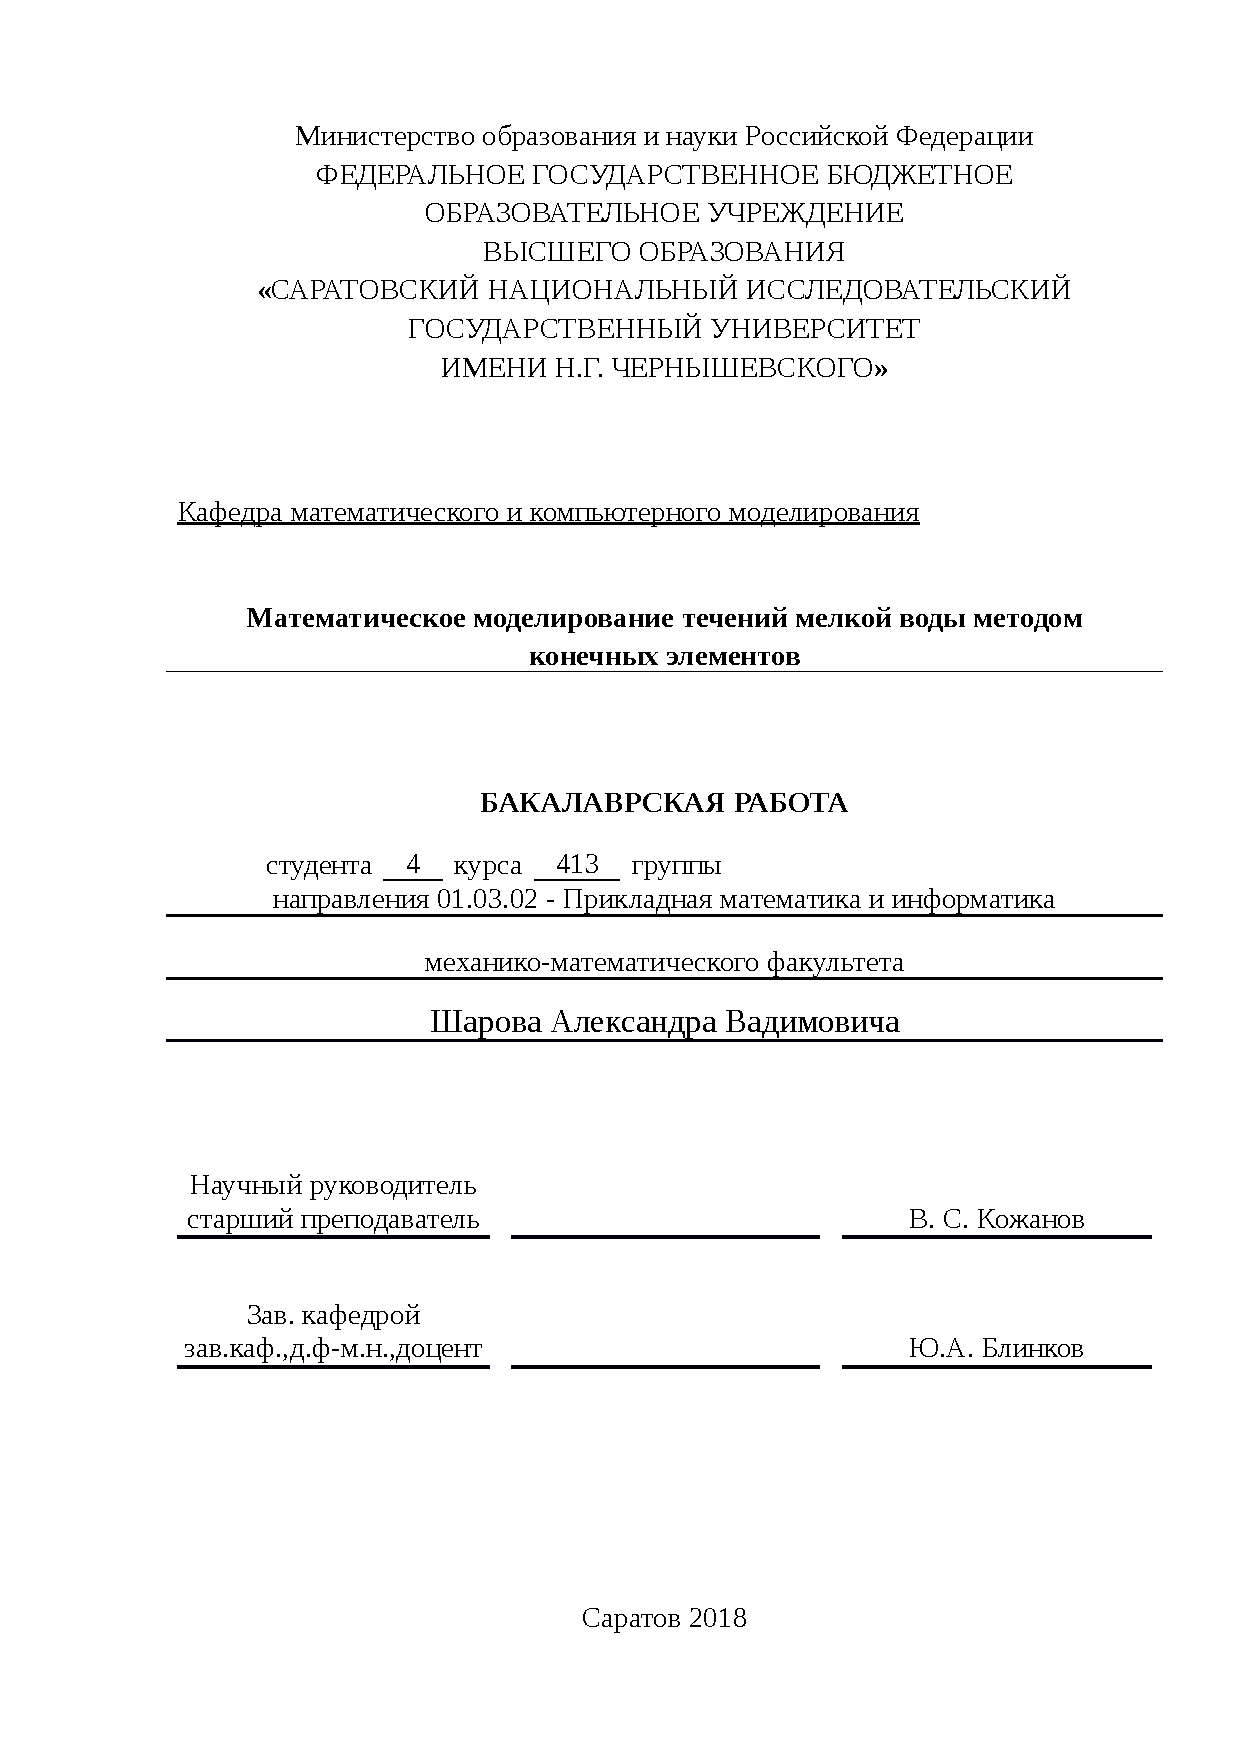
\includepdf[pages={1}]{titul/diploma.pdf}

\tableofcontents

\abbrevdef

\begin{enumerate}
\item МКЭ -- метод конечных элементов
\item КЭ -- конечный элемент
\item МВ -- мелкая вода
\item ГЖС -- газожидкостная смесь
\item POLY -- тип файла, в котором содержится список вершин и сегментов. Помимо этого, данный файл может содержать в себе информацию о пустотах и вогнутостях, а также некоторую дополнительную информацию\cite{bib:website:quake:triangle}
\item СУБД -- система управления базами данных
\item БД -- база данных
\item NoSQL -- термин, обозначающий ряд подходов, направленных на реализацию хранилищ баз данных, имеющих существенные отличия от моделей, используемых в традиционных реляционных СУБД с доступом к данным средствами языка SQL
\item Oracle RDBMS -- объектно-реляционная система управления базами данных компании Oracle
\item Нода кластера -- один компьютер в группе, объединённой высокоскоростными каналами связи и представляющей с точки зрения пользователя единый аппаратный ресурс
\item Docker -- программное обеспечение для автоматизации развёртывания и управления приложениями в среде виртуализации на уровне операционной системы
\end{enumerate}

\intro

Для корректного построения математических моделей и численных методов расчета течения жидкости важно знать, каким именно образом описываются основные процессы, происходящие в водоеме. Для этого строятся модели, которые учитывают основные характеристики течения в природной среде.

На данный момент во многих случаях не оправдывается применение более сложных математических моделей для исследования течений в прибрежных водах и озерах, чем модели, полученные путем применения осредненных по вертикали характеристик и основанные на численном решении двумерных уравнений -- уравнений мелкой воды.

Уравнения мелкой воды -- широко известное приближение, на основе которого проводится численное моделирование течений в реках и водоемах, в прибрежных зонах морей и океанов. Трехмерные решения данных уравнений являются нецелесообразными, так как они требуют намного большего количества исходной информации и машинного времени даже с учетом современных вычислительных мощностей.

При выводе данных уравнений предполагается, что среда представляет собой достаточно тонкий слой, глубина которого много меньше его продольного размера, поэтому вертикальной составляющей скорости можно пренебречь и полагать, что продольные скорости постоянны по толщине слоя.  Исходя из этого данное приближение успешно применяется для описания течений, где влияние на поток свободной поверхности и рельефа дна значительно.

Целью представленной бакалаврской квалификационной работы является построение и численная реализация математической модели на основе двумерных уравнений мелкой воды с помощью метода конечных элементов, который уже давно зарекомендовал\cite{bib:fem:nory} себя в таких областях, как механика деформируемого тела, электродинамика и, конечно же, гидродинамика. Данный метод является оптимальным для решения поставленной задачи, так как именно он дает возможность применять достаточно гибкую разбивку рассматриваемой области и при его использовании достаточно удовлетворить лишь главным граничным условиям. Для этой задачи требуется составить и решить систему дифференциальных уравнений с использованием метода конечных элементов. Предполагается, что глубина водоема постоянна, а сам водоем является однородным, то есть не рассматривается случай ГЖС. Необходимо учесть, что озеро подвержено влиянию ветра, а также требуется рассмотреть данную задачу с различными начальными параметрами и проанализировать полученные результаты. Похожая задача для уже решалась ранее, но рассматривался либо только стационарный случай\cite{bib:pankratov:2014:RTMV}, либо использовались другие методы\cite{bib:pankratov:2016:ANYMV}.

Актуальность данной работы обусловлена тем, что сейчас есть потребность в более точном и быстром решении уже решенных физических задач. Этой потребности отвечает появление новых быстродействующих систем и методов решения. Так, в данной бакалаврской работе была разработана параллельная реализация МКЭ для уравнений МВ, которая позволит более эффективно исследовать различные течения, которые могут быть описаны с помощью уравнений МВ.

В данной работе будут представлены основные определения и понятия для уравнений мелкой воды, которые позволят составить и решить поставленную задачу, состоящую из двух частей: аналитической и численной. Аналитически будут описаны течения жидкости при пренебрежении температурными эффектами, для которых широко используются классические уравнения Сен-Венана. После этого с помощью МКЭ была построена и рассчитана математическая модель МВ. В качестве реализации модели будет написана программа на языке Python\cite{bib:python:lutz:2013,bib:python:nm:2013}, которая выдает результаты решения системы уравнений мелкой воды, а также строит графики, наглядным образом отображающие полученные результаты.

 
\chapter{Вывод уравнений мелкой воды}

Запишем два основных уравнения для жидкости -- уравнение количества движения и уравнение неразрывности \cite{bib:fem:konor}:

\begin{equation}\label{eq:shallow_water:1}
-\frac{\partial p}{\partial x_k} + \frac{\partial \tau_{ik}}{\partial x_i} + \rho b_k = \frac{\partial}{\partial x_i}(\rho v_i v_k) + \frac{\partial}{\partial t}(\rho v_k);
\end{equation}

\begin{equation}\label{eq:shallow_water:2}
\frac{D\rho}{Dt}+\rho \frac{\partial v_i}{\partial x_i} =0.
\end{equation}

Если в \ref{eq:shallow_water:1} и \ref{eq:shallow_water:2} пренебречь температурными эффектами, получим:

\begin{equation}\label{eq:shallow_water:3}
-\frac{\partial p}{\partial x_k} + \frac{\partial \tau_{ik}}{\partial x_i} + \rho b_k = \frac{D(\rho v_k)}{Dt}
\end{equation}

\begin{equation}\label{eq:shallow_water:4}
\frac{\partial (\rho v_i)}{\partial t} + \frac{\partial \rho}{\partial t}=0,
\end{equation}

\noindentгде $p$ -- давление, оказываемое на единицу площади поверхности воды, $b_k$ -- массовые силы, приходящиеся на единицу массы, $v_k$ -- скорость частицы воды в направлении оси $x_k$, $\tau_{ik}$ -- вязкостные составляющие вектора напряжения, $\rho$ -- массовая плотность воды.

При математическом моделировании движения мелкой воды сложно применять данные уравнения вследствие наличия свободной поверхности, изменения границ во время приливов и отливов и большого количества переменных.

Данных трудностей можно избежать после ряда упрощений, в результате чего получаются уравнения мелкой воды. Первое упрощение состоит в том, что уравнение количества движения в проекции на ось $x_3$ записывается в виде:

\begin{equation}\label{eq:shallow_water:5}
-\frac{\partial p}{\partial x_3}=\rho g, 
\end{equation}

\noindentгде массовые силы отрицательны, поскольку действуют в направлении, противоположном оси $x_3$. При выводе формулы \ref{eq:shallow_water:5} пренебрегаем всеми членами, которые характеризуют ускорение, и соответствующими им напряжениями. Проинтегрируем выражение \ref{eq:shallow_water:5} и в результате получим:

\begin{equation}\label{eq:shallow_water:6}
p = \int\limits^\eta_{x_3} \rho g dx_3 = \rho g (\eta-x_3)+p_a,
\end{equation}

\noindent где $p_a$ -- атмосферное давление на поверхности воды,
$\eta$ -- возвышение свободной поверхности в соответствии с рисунком \ref{img:shallow_water:1}.

\begin{figure}[H]
\centerline{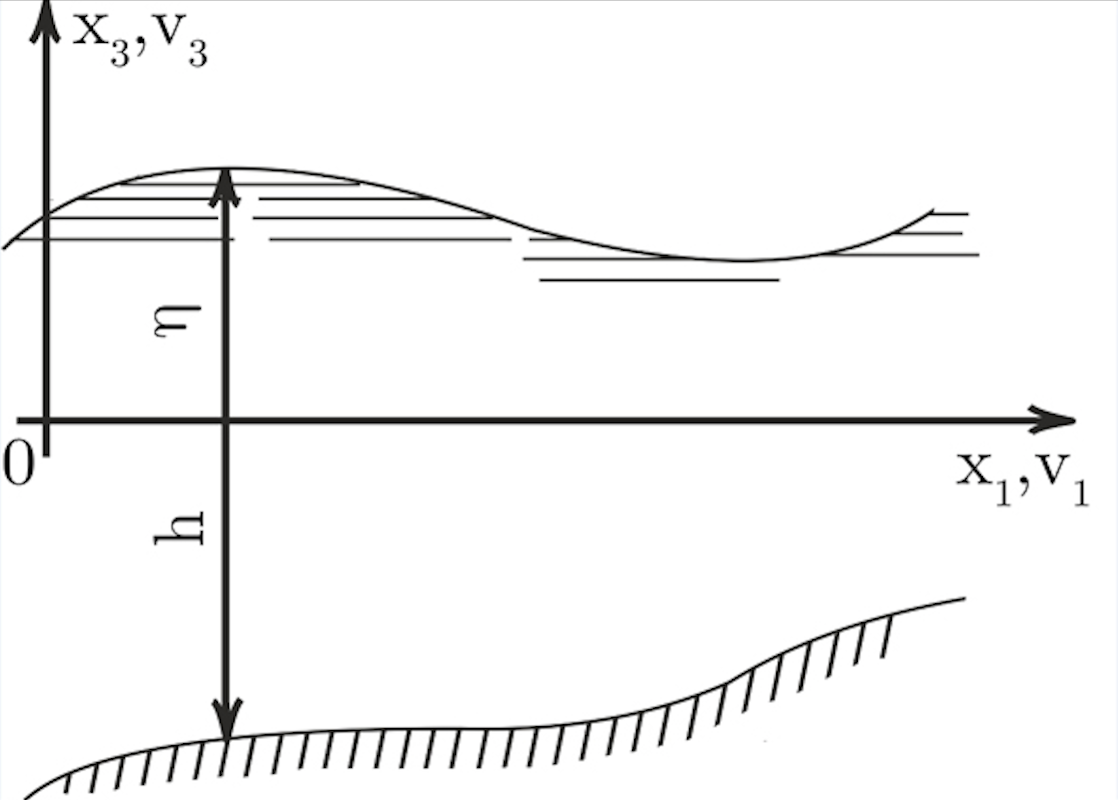
\includegraphics[width=0.5\linewidth]{images/shallow_water_1}}
\caption{Возвышение свободной поверхности.}
\label{img:shallow_water:1}
\end{figure}

Оставшиеся два уравнения количества движения по направлениям $x_1$ и $x_2$ останутся без изменений:

\begin{equation}\label{eq:shallow_water:7}
-\frac{\partial p}{\partial x_k} + \frac{\partial \tau_{ik}}{\partial x_i} + \rho b_k = \frac{D(\rho v_k)}{Dt}.
\end{equation}

\noindentПри $k=1$ выражение \ref{eq:shallow_water:7} дает проекцию на ось $x_1$, при $k=2$ -- на ось $x_2$. В выражении \ref{eq:shallow_water:7} величина $v$ -- средняя скорость, $\rho$ - переменная массовая плотность и $\tau$ -- сумма вязкостных и турбулентных напряжений.

Проинтегрируем выражения \ref{eq:shallow_water:4} и \ref{eq:shallow_water:7} по $x_3$. Для уравнения неразрывности это даст:

\begin{equation}\label{eq:shallow_water:8}
\int\limits^\eta_{-h} \bigg(\frac{\partial (\rho v_i)}{\partial x_i} + \frac{\partial \rho}{\partial t}\bigg) dx_3 =0,
\end{equation}

\noindentгде $h$ -- это глубина, измеряемая от базовой поверхности (в общем случае не горизонтальной).

Определим поток $q_k$ количества жидкости (массу жидкости, приходящуюся на единицу длины и времени):

\begin{equation}\label{eq:shallow_water:9}
q_i = \int\limits^\eta_{-h} \rho v_i dx_3 = \rho \int\limits^\eta_{-h} v_i dx_3.
\end{equation}

\noindentПредполагается, что $\rho(x_1, x_2)$ не зависит от $x_3$.

При интегрировании уравнения \ref{eq:shallow_water:8} необходимо использовать кинематическое условие и правило Лейбница \cite{bib:calc:zorich} для вычисления частной производной интеграла с переменными пределами. Согласно этому правилу:


\begin{equation}\label{eq:shallow_water:10}
\frac{\partial}{\partial x_1} \int\limits^{h_2(x_1,x_2)}_{h_1(x_1,x_2)} f(x_1, x_2, x_3) dx_3=\int\limits^{h_2(x_1,x_2)}_{h_1(x_1,x_2)} \frac{\partial f}{\partial x_1} dx_3 + f \bigg|_{h_2}  \frac{\partial h_2}{\partial x_1} + f \bigg|_{h_1} \frac{\partial h_2}{\partial x_1}.
\end{equation}

Аналогично для производной по $x_2$.

Кинематическое соотношение для свободной поверхности можно записать следующим образом:

\begin{equation}\label{eq:shallow_water:11}
v_3\bigg|_{x_2=\eta} = \frac{D\eta}{Dt} = \frac{\partial \eta}{\partial t} + v_1 \bigg|_{\eta} \frac{\partial \eta}{\partial x_1} + v_2 \bigg|_{\eta}\frac{\partial \eta}{\partial x_2}.
\end{equation}

\noindentПрименим формулы \ref{eq:shallow_water:9}-\ref{eq:shallow_water:11} к уравнению \ref{eq:shallow_water:8} и получим:

\begin{equation}\label{eq:shallow_water:12}
\frac{ \partial q_i}{\partial x_i} + \frac{\partial(\rho H)}{\partial t} = 0,
\end{equation}

\noindentгде $H=\eta+h$.

Чтобы проинтегрировать уравнение количества движения \ref{eq:shallow_water:7} по $x_3$, определим мгновенные скорости $v_1$, $v_2$:

\begin{equation}\label{eq:shallow_water:13}
\begin{aligned}
v_1 = \overline{v_1} (x_1, x_2, t) + v_1'(x_1, x_2, x_3, t);\\
v_2 = \overline{v_2} (x_1, x_2, t) + v_2'(x_1, x_2, x_3, t),
\end{aligned}
\end{equation}

\noindentгде величина $\overline{v}$ означает средние по вертикали скорости, а $v’$ -- отклонение от этих средних значений при различных значениях $x_3$.

\noindentСледовательно:

\begin{equation}\label{eq:shallow_water:14}
<v_k>=\int\limits^\eta_{-h} v_k dx_3 = \frac{1}{\rho} q_k, \; v_k=\frac{1}{H}<v_k>,
\end{equation}

\noindentтак как $<v_k’> = 0$, где знак $<>$ означает среднее значение стоящее внутри величины.

Будем предполагать, что массовые силы обусловлены только эффектом Кориолиса. Таким образом получаем:

\begin{equation}\label{eq:shallow_water:15}
b_1 = \rho f v_2, \; b_2 = - \rho f v_1.
\end{equation}

\noindentПредположим, что наклоны поверхности и дна малы по сравнению с единицей, тогда составляющие внутреннего напряжения можно аппроксимировать следующим образом в соотвествии с рисунком \ref{img:shallow_water:2}:

\begin{equation}\label{eq:shallow_water:16}
\begin{aligned}
 \tau_1\bigg|_s \approx \bigg\{ -\tau_{11}\frac{\partial \theta}{\partial x_1} -\tau_{12}\frac{\partial \theta}{\partial x_2} +\tau_{13}\bigg\}, \\
\tau_1\bigg|_b \approx \bigg\{ \tau_{11}\frac{\partial h}{\partial x_1} +\tau_{12}\frac{\partial h}{\partial x_2} -\tau_{13}\bigg\}.
\end{aligned}
\end{equation}

\noindentАналогичные значения можно выписать для величин $\tau_2|_s$ и $\tau_2|_b$.

\begin{figure}[H]
\centerline{

\includegraphics[width=0.5\linewidth]{images/shallow_water_2}}
\caption{Силы, действующие на свободную поверхность.}
\label{img:shallow_water:2}
\end{figure}


Величины $\tau_2|_s$ и $\tau_2|_b$ можно интерпретировать как компоненты внешней силы, приложенные к поверхности и дну.

Подставим теперь соотношения \ref{eq:shallow_water:13} - \ref{eq:shallow_water:15} в уравнения количества движения, проинтегрированные по $x_3$, и дополнительно используем правило Лейбница\cite{bib:calc:zorich} и кинематическое условие \ref{eq:shallow_water:11}. Тогда:

\begin{equation}\label{eq:shallow_water:17}
\begin{aligned}
\frac{\partial q_1}{\partial t} + \frac{\partial}{\partial x_1} \bigg(\frac{q_1^2}{H}\bigg)+\frac{\partial }{\partial x_2}\bigg(\frac{q_1 q_2}{H}\bigg) = -\frac{\partial N_p}{\partial x_2} + \frac{\partial N_{11}}{\partial x_1} + \frac{\partial N_{12}}{\partial x_2} +\\+ fq_2 + p\bigg|_s \frac{\partial \eta}{\partial x_1} + \tau_1\bigg|_s+p\bigg|_b\frac{\partial h}{\partial x_1} - \tau_1\bigg|_b; \\
\frac{\partial q_2}{\partial t} + \frac{\partial}{\partial x_1} \bigg(\frac{q_1 q_2}{H}\bigg)+\frac{\partial }{\partial x_2}\bigg(\frac{q_2^2}{H}\bigg) = -\frac{\partial N_p}{\partial x_2} + \frac{\partial N_{22}}{\partial x_2} + \frac{\partial N_{21}}{\partial x_1} +\\+ fq_1 + p\bigg|_s \frac{\partial \eta}{\partial x_2} + \tau_2\bigg|_s+p\bigg|_b\frac{\partial h}{\partial x_2} - \tau_2\bigg|_b,
\end{aligned}
\end{equation}

\noindentгде

\begin{equation}\label{eq:shallow_water:18}
\begin{aligned}
N_p = <p> = \int\limits^\eta_{-h} pdx_3=\rho g \frac{H^2}{2} + Hp_a; \\
N_{11} = <\tau_{11}>-<pv_1'v_1'>; \\
N_{22} = <\tau_{22}>-<pv_2'v_2'>; \\
N_{12} = <\tau_{12}>-<pv_1'v_2'>;
\end{aligned}
\end{equation}

\noindentБолее того, элементы $N_{ik}$ могут быть аппроксимированы следующими выражениями:

\begin{equation}\label{eq:shallow_water:19}
\begin{aligned}
N_{11} \approx 2 \varepsilon_{11}\frac{\partial q_1}{\partial x_1}; \\
N_{22} \approx 2 \varepsilon_{22}\frac{\partial q_2}{\partial x_2}; \\
N_{12} \approx \varepsilon_{12}\bigg(\frac{\partial q_2}{\partial x_1}+\frac{\partial q_1}{\partial x_2}\bigg),
\end{aligned}
\end{equation}

\noindentгде $\varepsilon_{ik}$ обобщенные коэффициенты вихревой вязкости. Для изотропного характера течения $\varepsilon_{11}=\varepsilon_{22}=\varepsilon_{12}=\varepsilon.$

Касательные напряжения на дне обычно определяются соотношениями:

\begin{equation}\label{eq:shallow_water:20}
\begin{aligned}
\tau_1\bigg|_b = \frac{g}{c^2} \frac{1}{\rho} \frac{q_1\sqrt{(q_1^2+q_2^2)}}{H^2}; \\
\tau_2\bigg|_b = \frac{g}{c^2} \frac{1}{\rho} \frac{q_2\sqrt{(q_1^2+q_2^2)}}{H^2},
\end{aligned}
\end{equation}

\noindentгде $g$ -- ускорение силы тяжести, $c$ -- коэффициент трения, $\rho$ -- плотность воды. 

Составляющие напряжения трения на поверхности воды обычно обусловлены действием ветра и могут быть найдены по формулам:

\begin{equation}\label{eq:shallow_water:21}
\begin{aligned}
\tau_1\bigg|_s=\gamma^2\rho_aW^2\cos(\theta);\\
\tau_2\bigg|_s=\gamma^2\rho_aW^2\sin(\theta),
\end{aligned}
\end{equation}

\noindentгде $\gamma^2$ -- коэффициент ветрового напряжения, $\rho_a$ -- плотность воздуха, $W$ -- скорость ветра, $\theta$ -- угол между осью $x_1$ и направлением ветра.

Уравнения \ref{eq:shallow_water:17} перепишем в виде:


\begin{equation}\label{eq:shallow_water:22}
\begin{aligned}
\dfrac{\partial q_1}{\partial t} + \dfrac{\partial}{\partial x_1} \bigg(\dfrac{q_1^2}{H}\bigg)+\dfrac{\partial }{\partial x_2}\bigg(\dfrac{q_1 q_2}{H}\bigg) = \dfrac{\partial}{\partial x_1} (N_{11}-N_p) + \dfrac{\partial N_{12}}{\partial x_2} + B_1; \\
\dfrac{\partial q_2}{\partial t} + \dfrac{\partial}{\partial x_1} \bigg(\dfrac{q_1 q_2}{H}\bigg)+\dfrac{\partial }{\partial x_2}\bigg(\dfrac{q_2^2}{H}\bigg) = \dfrac{\partial}{\partial x_2} (N_{22}-N_p) + \dfrac{\partial N_{12}}{\partial x_2} + B_2,
\end{aligned}
\end{equation}

\noindentгде

\begin{equation*}
\begin{aligned}
B_1=fq_2+\gamma^2\rho_aW^2\cos(\theta)-\bigg(\dfrac{g}{c^2}\bigg)\dfrac{1}{\rho}\dfrac{q_1\sqrt{(q_1^2+q_2^2)}}{H^2} + p_a \dfrac{\partial H}{\partial x_1} + \rho gH\dfrac{\partial h}{\partial x_1}; \\
B_2=-fq_1+\gamma^2\rho_aW^2\sin(\theta)-\bigg(\dfrac{g}{c^2}\bigg)\dfrac{1}{\rho}\dfrac{q_2\sqrt{(q_1^2+q_2^2)}}{H^2} + p_a \dfrac{\partial H}{\partial x_2} + \rho gH\dfrac{\partial h}{\partial x_2}.
\end{aligned}
\end{equation*}

Для решения окончательной системы уравнений \ref{eq:shallow_water:22}, дополненных условием \ref{eq:shallow_water:12}, необходимо установить требуемые граничные условия. Будем считать, что граница $S$ состоит из двух частей: твердой границы $S_1$ и жидкой $S_2$, представляющей границу рассматриваемого водоема с открытым морем в соотвествии с рисунком \ref{img:shallow_water:3}.

\begin{figure}[H]
\centerline{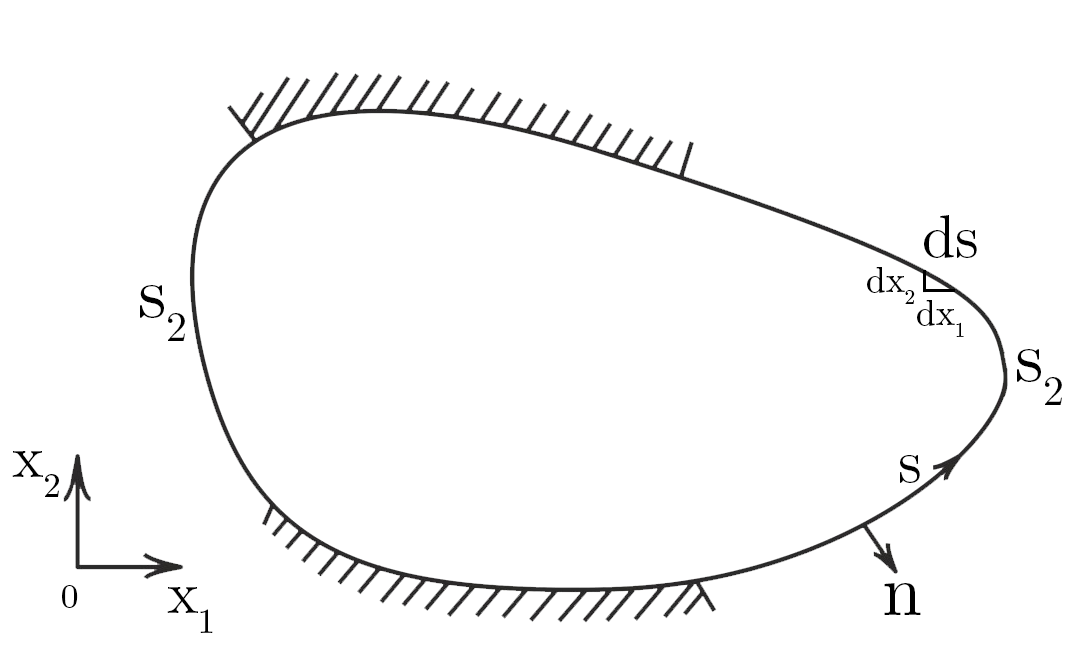
\includegraphics[width=0.5\linewidth]{images/shallow_water_3}}
\caption{Водоём с изображенными границами.}
\label{img:shallow_water:3}
\end{figure}

В системе координат $s-n$, связанной с границей течения, расход массы жидкости можно записать через $q_s$ и $q_n$:

\begin{equation}\label{eq:shallow_water:24}
\begin{aligned}
q_n=\int\limits^\eta_{-h} \rho v_n dx_3= \alpha_{n1}q_1+\alpha_{n2}q_2; \\
q_s=\int\limits^\eta_{-h} \rho v_s dx_3= -\alpha_{n2}q_1+\alpha_{n1}q_2,
\end{aligned}
\end{equation}

\noindentгде $\alpha_{n1}=\cos(\overline{n},x_1); \alpha_{n2}=\cos(\overline{n},x_2).$

Для установления результирующих сил можно воспользоваться формулами:

\begin{eqnarray}
N_{n1}=\alpha_{n1}(N_{11}-N_{p})+\alpha_{n2}N_{12}; \nonumber\\
N_{n2}=\alpha_{n1}N_{12}+\alpha_{n2}(N_{22}-N_{p}).
\end{eqnarray}

По значениям $N_{n1}$ и $N_{n2}$ определяется нормальная и касательная составляющие результирующей силы для наклонной площадки:

\begin{eqnarray}
N_{nn}=\alpha_{n1}N_{n1}+\alpha_{n2}N_{n2}; \nonumber\\
N_{ns}=\alpha_{n2}N_{n1}+\alpha_{n1}N_{n2}.
\end{eqnarray}

Если же в исследуемую акваторию впадает река, то на $S_1$:

\begin{eqnarray}
q_n=\overline{q_n}=|q|; \nonumber\\
q_s=0,
\end{eqnarray}

\noindentгде $|q|$ - поток втекающей
реки. 

На жидкой границе $ S_2 $ необходимо задать нормальные и касательные силы:

\begin{eqnarray}
N_{nn}=\overline{N_{nn}}; \nonumber\\
N_{ns}=\overline{N_{ns}}.
\end{eqnarray}

\noindentНо так как слагаемыми, учитывающими вихревую вязкость в уравнении \ref{eq:shallow_water:22} можно пренебречь, то касательные силы или скорости не могут быть заданы. Таким образом, граничные условия сводятся к следующим:

\begin{eqnarray}
q_n=0 \; \text{или} \; q_n=\overline{q_n} \; \text{на} \; S_1\nonumber\\
N_{nn}=\overline{N_{nn}}=-N_p \; \text{на} \; S_2.
\end{eqnarray}

\chapter{Постановка задачи}

Рассматривается течение мелкой воды в закрытом водоеме при учете влияния на этот водоем ветра. Это явление описывается системой дифференциальных уравнений в частных производных\cite{bib:calc:yurko:2004}, которая состоит из двух уравнений мелкой воды и уравнения неразрывности:

\begin{eqnarray}\label{eq:task:1}
\begin{cases}
\dfrac{ \partial q_i}{\partial x_i} + \dfrac{\partial(\rho H)}{\partial t} = 0 \\
\dfrac{\partial q_1}{\partial t} + \dfrac{\partial}{\partial x_1} \bigg(\dfrac{q_1^2}{H}\bigg)+\dfrac{\partial }{\partial x_2}\bigg(\dfrac{q_1 q_2}{H}\bigg) = \dfrac{\partial}{\partial x_1} (N_{11}-N_p) + \dfrac{\partial N_{12}}{\partial x_2} + B_1 \\
\dfrac{\partial q_2}{\partial t} + \dfrac{\partial}{\partial x_1} \bigg(\dfrac{q_1 q_2}{H}\bigg)+\dfrac{\partial }{\partial x_2}\bigg(\dfrac{q_2^2}{H}\bigg) = \dfrac{\partial}{\partial x_2} (N_{22}-N_p) + \dfrac{\partial N_{12}}{\partial x_2} + B_2,
\end{cases}
\end{eqnarray}

\noindentгде

\begin{equation}\label{eq:task:2}
\begin{aligned}
B_1=fq_2+\gamma^2\rho_aW^2\cos(\theta)-\bigg(\dfrac{g}{c^2}\bigg)\dfrac{1}{\rho}\dfrac{q_1\sqrt{(q_1^2+q_2^2)}}{H^2} + p_a \dfrac{\partial H}{\partial x_1} + \rho gH\dfrac{\partial h}{\partial x_1}; \\
B_2=-fq_1+\gamma^2\rho_aW^2\sin(\theta)-\bigg(\dfrac{g}{c^2}\bigg)\dfrac{1}{\rho}\dfrac{q_2\sqrt{(q_1^2+q_2^2)}}{H^2} + p_a \dfrac{\partial H}{\partial x_2} + \rho gH\dfrac{\partial h}{\partial x_2}.
\end{aligned}
\end{equation}

В системе задействованы следующие переменные физические величины:

\begin{threeparttable}
\begin{longtable}[H]{lp{0.7\linewidth}}
{$\rho$} -- плотность воды & 1000 [кг/м\textsuperscript3] \\
{$c$} -- коэффициент трения Шэзи & 10 [м\textsuperscript{1/2}с\textsuperscript{-1}] \\
{$g$} -- ускорение свободного падения & 9,832 [м/с\textsuperscript{2}] \\
{$\gamma^2$} -- коэффициент ветрового напряжения & 0.002 \\

{$p_a$} -- атмосферное давление на поверхности воды & $10^5$ [Па] \\
{$\rho_a$} -- плотность воздуха & 1,2754 [кг/м\textsuperscript3] \\
{$f$} -- сила Кориолиса & $0.973 \cdot 10^{-4}$ [1/с] \\
\end{longtable} 
\end{threeparttable}

Также в системе используются следующие переменные:

\begin{threeparttable}
\begin{longtable}[H]{lp{0.7\linewidth}}
{$W$} -- скорость ветра & [м/с] \\
{$\theta$} -- угол между $x_1$ и направлением ветра & \\
{$h$} -- возвышение свободной поверхности & [м]
\end{longtable} 
\end{threeparttable}


Для данного двумерного случая системы дифференциальных уравнений требуется найти решение с помощью метода конечных элементов. Реализация должна работать с любой произвольно заданной областью. В качестве примеров таких областей должны быть как искусственно вырытые пруды, так и реальные озера. 

Так как задача рассматривается двумерная, то КЭ будет представлять из себя треугольник. Простые двумерные области разбиваются на квадраты, которые впоследствии разбиваются на треугольники. В случае более сложной геометрии триангуляция рассматриваемой области осуществляется с помощью более сложных алгоритмов, которые необходимо рассмотреть перед решением поставленной задачи, для того чтобы корректно генерировать сетку, на которой будет найдено решение поставленной задачи. В следующем разделе рассмотрены два основных алгоритма триангуляции, дающие оптимальные разбиения исходной области.

\chapter{Триангуляция двумерной области}

В геометрии триангуляция дискретного множества точек $P\subset {\mathbb  {R}}^{{n+1}}$ в наиболее общем значении — это разбиение  выпуклой оболочки некоторого набора точек, которое представляет собой планарный граф\cite{bib:triangle:delone}. Одна из фигур разбиения является выпуклой оболочкой разбиваемого множества, а остальные симплексами --  геометрическими фигурами, которые являются $n-$мерным обобщением треугольника. В любой триангуляции ($T$) формально должны выполняться следующие свойства:

	1. любые два симплекса в T пересекаются в общей грани ребра или вершины или вообще не пересекаются;

	2. множество точек, являющихся вершинами симплексов разбиения, совпадает с множеством $P$;
	
	3. нельзя добавить ни одного нового ребра в граф без нарушения планарности.

Одно и то же множество можно триангулировать разными способами. Триангуляция дает тем лучшую аппроксимацию, чем больше её минимальный угол, при этом формируемые симплексы стремятся к равноугольности. Очень важна максимизация минимального угла в вычислительных задачах, когда точность производимых вычислений очень сильно зависит от размера минимального угла триангуляции. Наилучшей в этом смысле триангуляцией является триангуляция Делоне. Простейшим способом её построения является инкрементальный алгоритм, работающий за $o(n^2)$ операций, но он не поддерживает вырожденные случаи, когда $4$ точки из множества лежат на одной окружности: в этом случае триангуляция Делоне не уникальна, и способов разбиения существует несколько, но минимальные углы этих триангуляций равны. Иногда даже минимальный угол триангуляции Делоне оказывается слишком малым для устойчивой работы использующего её алгоритма, и тогда можно произвести улучшение, используя алгоритм Рапперта [J. Ruppert]. При этом будут добавлены новые вершины триангуляции, а также образованы дополнительные треугольники. Стабильность численного алгоритма (метода конечных элементов, к примеру) может возрасти многократно за счет появления нижней границы для углов. 

\section{Алгоритм Рапперта [Jim Ruppert]}

Алгоритм Рапперта [J. Ruppert], или же усовершенствованный алгоритм Делоне, довольно новый, он был опубликован в 1994 году. Данный алгоритм адаптирован для МКЭ, а это значит, что он удовлетворяет всем требованиям, которые предъявляются к конечно-элементным сеткам, а именно:

1. треугольники не должны быть сильно вытянутыми, так как наличие таких треугольников отрицательно сказывается на точности результатов расчета;

2. должна быть учтена геометрия рассматриваемой области, и в местах со сложной геометрией сетка должна сгущаться.

Если говорить точнее, алгоритм Рапперта [J. Ruppert] не является алгоритмом генерации сеток. Он является лишь алгоритмом улучшения качества сетки, от чего и произошло название. В общем случае входными данными для него будут являться геометрия конструкции в виде замкнутых полигонов и первичное разбиение конструкции на треугольники. 

При описании алгоритма Рапперта [J. Ruppert] следует ввести следующую терминологию:
\begin{itemize}
\item Элемент по смыслу совпадает с конечным элементом. Это элементарная часть пространства, на множество которых мы хотим разбить более сложную область этого пространства;

\item Узел — точка в которой сходятся грани и соприкасаются несколько элементов;

\item Сегмент — это отрезок, соединяющий две соседние точки лежащие на границе области разбиения; Другими словами, этот отрезок принадлежит контурам области;

\item Грань — это отрезок, по которому граничат два соприкасающихся треугольника;

\item Включенная точка — любая вершина текущей сетки, находящаяся внутри окружности, радиусом которой является любой сегмент;

\item <<Неправильный треугольник>> — треугольник, не удовлетворяющий глобальным условиям, которые накладываются на генерируемую сетку;

\item Вытянутый треугольник — треугольник, имеющий одну сторону, намного отличающуюся от других двух. То есть треугольник слишком вытянут вдоль некоторой прямой.
\end{itemize}

Алгоритм опирается на две базовые процедуры: 

\begin{enumerate}

\item Разбиение неправильного треугольника с введением нового узла.

\begin{enumerate}

\item Вычисляются координаты центра окружности, описанной вокруг треугольника, подлежащего разбиению

\item В найденную точку добавляется новый узел

\item Удаляется треугольник, подлежащий разбиению, и прилегающие к нему треугольники, а затем добавляются новые в соответствии с рисунком \ref{img:triangle:1}

\end{enumerate}

\begin{figure}[H]
\centerline{
\includegraphics[width=0.5\linewidth]{images/puppert_1}}
\caption{Разбиение <<неправильного>> треугольника.}
\label{img:triangle:1}
\end{figure}

\item Разбиение сегмента, принадлежащего границе области разбиения с введением нового узла. 

\begin{enumerate}

\item Если в окружность, диаметром которой является сегмент, принадлежащий границе области разбиения, попадает точка, не принадлежащая этому сегменту, то сегмент делится на две части;

\item Удаляется треугольник, которому принадлежал первоначальный сегмент, и добавляются два новых треугольника в соответствии с рисунком \ref{img:triangle:2}.

\end{enumerate}
\end{enumerate}


\begin{figure}[H]
\centerline{
\includegraphics[width=0.8\linewidth]{images/puppert_2}}
\caption{Разбиение <<неправильного>> сегмента посередине и добавление двух новых треугольников.}
\label{img:triangle:2}
\end{figure}


Принцип работы алгоритма состоит в цикле определения <<неправильных>> треугольников. В каждом треугольнике сетки определяется минимальный угол и, затем сравниваются минимальные углы для всех треугольников с целью нахождения минимального угла сетки. Другими словами, минимальный угол в сетке равен минимально возможному углу, который образован двумя сегментами, либо двумя гранями, либо сегментом и гранью, имеющими общий узел.

Критерий минимального угла автоматически обеспечивает сгущение сетки вблизи мелких подробностей: отверстий, углов и вырезов. 

Все описанные процедуры выполняются в определенной последовательности, они имеют разный приоритет. Общая схема работы алгоритма следующая:

\begin{enumerate}

\item Производится поиск включенной точки перебором всех точек и сегментов (только сегментов, но не граней).

\item Если такая точка найдена, то над сегментом, который включает ее, выполняется процедура деления сегмента пополам и производится возврат на шаг 1. Если включенных точек не было найдено, то алгоритм переходит на следующий шаг.

\item Производится поиск треугольника с минимальным углом.

\item Если минимальный угол меньше заданного параметра, то над треугольником, и его содержащим производится процедура деления и производится возврат на шаг 1. В противном случае происходит переход на следующий шаг.

\item Производится поиск треугольника максимальной площадью.

\item Если максимальная площадь больше заданного параметра, то над таким треугольником производится процедура деления и производится возврат на шаг 1. В противном случае происходит переход на следующий шаг.

\item Все условия удовлетворены. Конец работы алгоритма

\end{enumerate}


Автор в своей работе \cite{bib:triangle:ruppert} приводит строгие математические доказательства, гарантирующие правильную работу алгоритма при минимальном угле $\alpha < 20^{\circ}$. Данный алгоритм имеет ряд теоретических и практических преимуществ для генерации сетки.  Для не острого ввода и минимального угла порога около $20.70^{\circ}$ алгоритм гарантированно завершает работу и создает сетку оптимального размера с постоянным коэффициентом, а также  дает теоретически подтвержденные гарантии качества получаемой с его помощью сетки.

\section{Алгоритм Чу [L. Paul Chew]}

В некоторых случаях в алгоритме Рапперта [J. Ruppert] получаются слишком большие сегменты, а для МКЭ очень хорошо иметь как можно более мелкие элементы в сетке. Для того чтобы этого избежать, был разработан алгоритм Чу [L. Chew], в котором сетка получается мельче за счет того, что он более консервативен в отношении разбиения на сегменты, когда граница угла меньше $30^{\circ}$. Главное преимущество данного алгоритма по сравнению с алгоритмом Рапперта [J. Ruppert] состоит в том, что КЭ в сетке получаются с углом до $28.6^{\circ}$, что является несомненным плюсом, так как элементы в сетке получаются приблизительно одинаковые. Алгоритм построен на более сложной теоретической базе \cite{bib:triangle:chew}, и главное его отличие от алгоритма Рапперта в том, что Рапперт только гарантирует хорошее разбиение и угол меньший, чем $20.7^{\circ}$, а Чу обязательно даст хорошее разбиение, правда, с углом до $26.5^{\circ}$. На практике данные алгоритмы дают примерно одинаковые разбиения, но алгоритм Чу является более популярным среди разработчиков математических пакетов.

\chapter{Метод конечных элементов в двумерной области}

Метод конечных элементов \cite{bib:fem:pankratov, bib:fem:zenkevich} -- численный метод решения дифференциальных уравнений в частных производных, возникающими при решении задач прикладной физики.
	В его основе лежат две главные идеи: дискретизация исследуемого объекта и кусочно-элементная аппроксимация исследуемых функций (в физической интерпретации - температуры, давления, перемещения и т.д.).

Идея состоит в том, что область, в которой ищется решение дифференциальных уравнений, разбивается на конечное количество элементов. В каждом из элементов произвольно выбирается вид аппроксимирующей функции. Вне своего элемента аппроксимирующая функция равна нулю. Значения функций в узлах являются решением задачи и заранее неизвестны. Коэффициенты аппроксимирующих функций обычно ищутся из условия равенства значения соседних функций на границах между элементами (в узлах). Затем эти коэффициенты выражаются через значения функций в узлах элементов. Составляется система уравнений. Количество уравнений равно количеству неизвестных значений в узлах, на которых ищется решение исходной системы, и прямо пропорционально количеству элементов. Так как каждый из элементов связан с ограниченным количеством соседних, система уравнений имеет разрежённый вид, что упрощает её решение. 

Если говорить в матричных терминах, то собираются так называемые матрицы жёсткости и масс. Далее на эти матрицы накладываются граничные условия (например, при условиях Неймана в матрицах не меняется ничего, а при условиях Дирихле из матриц вычёркиваются строки и столбцы, соответствующие граничным узлам, так как в силу краевых условий значение соответствующих компонент решения известно). После собирается система уравнений, тип которых может различаться в зависимости от поставленной задачи. Они могут быть как алгебраическими, так и дифференциальными. После того как система получена, она решается любым из доступных методов.

Основное отличие МКЭ от классических алгоритмов вариационных принципов и от методов невязок заключается в выборе базисных функций. Они берутся в виде кусочно-непрерывных функций, которые обращаются в ноль всюду, кроме ограниченных подобластей, являющихся конечными элементами. Это в свою очередь ведет к разреженной структуре матрицы коэффициентов разрешающей системы уравнений.

Главные достоинства МКЭ состоят в следующем:

1. исследуемые объекты могут иметь любую форму и различную физическую природу, это твёрдые тела, жидкости, газы, электромагнитные среды;

2. конечные элементы могут иметь различную криволинейную форму и различные размеры;

3. можно исследовать однородные и неоднородные, изотропные и анизотропные тела с линейными и нелинейными свойствами;

4. можно решать как стационарные, так и нестационарные задачи;

5. можно моделировать любые граничные условия;

6. вычислительный алгоритм, представленный в матричной форме, формально единообразен для различных физических задач и для задач различной размерности. Это удобно для вычисления на компьютере, так как методология не меняется и фактически используется единая программа численного решения;

7. на одной и той же сетке конечных элементов можно решать различные физические задачи, что облегчает анализ связанных между собой задач;

8. разрешающая система уравнений имеет разреженную симметричную ленточную матрицу жёсткости, что ускоряет вычислительный процесс.

Перед тем как рассматривать метод конечных элементов, рассмотрим метод взвешенных невязок, который является частным случаем метода конечных элементов с одним элементом.

\section{Метод взвешенных невязок}

Рассмотрим дифференциальное уравнение вида

\begin{equation}\label{eq:fem:1}
 \mathcal A= \mathcal L\phi + p=0
\end{equation}

\noindentв некоторой области $\Omega$.

Здесь $\mathcal L$ -- некоторый линейный дифференциальный оператор, а $p$ не зависит от неизвестной функции $\phi$.

Решение уравнения \ref{eq:fem:1} должно удовлетворять условию

\begin{equation}\label{eq:fem:2}
\mathcal B = \mathcal M \phi+r=0
\end{equation}

\noindentна замкнутой кривой $\Gamma$, ограничивающей область $\Omega$.

Здесь $\mathcal M$ -- соотвествующий линейный дифференциальный оператор, а $r$ не зависит от неизвестной функции $\phi$.

Построим аппроксимацию для решения $\phi$, которая на граничной кривой $\Gamma$ принимает те же значения, что и $\phi$. Если найти некоторую функцию $\psi$, принимающую одинаковые с $\phi$ значения на $\Gamma$, т.е. $\psi|_\Gamma= \phi|_\Gamma$, и ввести систему линейно независимых базисных функций $\{N_m; m = 1,2, \dots, N\}$, то на $\Omega$ можно предложить следующую аппроксимацию $\hat{\phi}$ для $\phi$: 

\begin{equation}\label{eq:fem:3}
\phi \approx \hat\phi = \psi + \sum\limits_{m=1}^{M} a_mN_m,
\end{equation}

\noindentгде $a_m, m= \overline{1,M}$ -- некоторые параметры, вычисляемые так, чтобы получить хорошее приближение, а функция $\psi$ и базисные функции $N_m$ выбраны таким образом, что

\begin{equation}\label{eq:fem:4}
 \mathcal M\psi=-r, \; \mathcal M N_m=0, \; m=\overline{1,M} \; \text{на} \; \Gamma,
\end{equation}

\noindentи поэтому $\phi$ автоматически удовлетворяет краевым условиям \ref{eq:fem:2} при произвольных коэффициентах $a_m$. Отметим, что система базисных функций (которые также называют функциями формы) должна быть выбрана так, чтобы гарантировать улучшение аппроксимации при возрастании числа базисных функций для $M$.

Для того чтобы найти аппроксимации производных от $\phi$, продифференцируем \ref{eq:fem:3} и получим:


\begin{gather}
\phi \approx \hat\phi = \psi + \sum\limits_{m=1}^{M} a_mN_m,\nonumber\\
\frac{\partial \phi}{\partial x} \approx \frac{\partial \hat\phi}{\partial x}=\frac{\partial \psi}{\partial x}+\sum\limits_{m=1}^{M} a_m\frac{\partial N_m}{\partial x},\nonumber\\
\frac{\partial^2 \phi}{\partial x^2} \approx \frac{\partial^2 \hat\phi}{\partial x^2}=\frac{\partial^2 \psi}{\partial x^2}+\sum\limits_{m=1}^{M} a_m\frac{\partial^2 N_m}{\partial x^2} \nonumber
\end{gather}

\noindentи т.д.

Так как построенное разложение \ref{eq:fem:3} удовлетворяет краевым условиям \ref{eq:fem:2}, то для получения аппроксимации искомой функции $\phi$ осталось гарантировать, что $\hat\phi$ -- приближённое решение уравнения \ref{eq:fem:1}. Для этого вначале введём невязку $R_\Omega$ в аппроксимации, определяемую по формуле:

\begin{equation}\label{eq:fem:5}
R_\Omega=A(\hat\phi)=\mathcal L \hat\phi+p=\mathcal L\psi+\bigg(\sum\limits_{m=1}^{M} a_m \mathcal L N_m\bigg) +p.
\end{equation}

Чтобы уменьшить эту невязку, потребуем равенства нулю соответствующего числа интегралов от погрешности \cite{bib:calc:zorich}, взятых с различными весами, т.е.

\begin{equation}\label{eq:fem:6}
\int_\Omega W_l R_\Omega d\Omega = \int_\Omega W_l \bigg\{\mathcal L \psi +\bigg(\sum\limits_{m=1}^{M} a_m \mathcal L N_m\bigg) +p \bigg\} d\Omega =0; \; l=\overline{1,M},
\end{equation}

\noindentгде $\{W_l:l=1,2,\dots,M\}$ -- это множество линейно независимых весовых (или пробных) функций.

Таким образом, система уравнений метода взвешенных невязок \ref{eq:fem:6} сводится к системе линейных алгебраических уравнений для неизвестных коэффициентов $a_m$, которую можно записать следующим образом:

\begin{equation}\label{eq:fem:7}
Ka=f,
\end{equation}

\noindentгде

\begin{gather}
a = (a_1,a_2,\dots, a_M)^T, \\
K_{lm}=\int_\Omega W_l \mathcal L N_m  d\Omega, \; l,m=\overline{1,M}; \\
f_l=-\int_\Omega W_l p d \Omega-\int_\Omega W_l \mathcal L \psi d \Omega \; l,m=\overline{1,M}.
\end{gather}

\noindentВычислив элементы матрицы $K$ и столбца свободных членов $f$ и решив затем полученную систему, мы найдем $a_m$, где $m=\overline{1,M}$, и тем самым закончим процесс построения приближенного решения \ref{eq:fem:1}.

\section{Метод конечных элементов}
В методе взвешенных невязок предполагалось, что базисные функции $N_m$ определены одним выражением на всей области $\Omega$. При этом интегралы в аппроксимирующем уравнении \ref{eq:fem:5} вычисляются по всей области.

С другой стороны, область $\Omega$ можно разбить на несколько непересекающихся подобластей (конечных элементов $\Omega^e$), которые могут иметь различную форму и размеры. В результате разбивки создается сетка из границ элементов:

$$\Omega=\bigcup\limits_{e=1}^E\Omega^{e}.$$


\noindentПересечение границ областей $\Omega^{e}$ образуют узлы. Выбор типа и размера КЭ напрямую зависит от рассматриваемой задачи.

После того как мы разбили рассматриваемую область $\Omega$ сеткой конечных элементов, можно аппроксимировать решение уравнения отдельно для каждой подобласти $\Omega^{e}$, где базисные функции могут быть определены различным образом для каждой из подобластей. В этом случае определённые интегралы, входящие в аппроксимирующие уравнения, можно посчитать просуммировав, вклады по каждому элементу:

\begin{gather}
\int_\Omega W_l R_\Omega d\Omega = \sum\limits_{e=1}^E\int_{\Omega^{e}} W_l R_\Omega d\Omega^e, \nonumber\\
\int_\Gamma \overline{W_l} R_\Gamma d\Gamma = \sum\limits_{e=1}^E\int_{\Gamma^{e}} W_l R_\Gamma d\Gamma^e.
\end{gather}

\noindentВ данных интегралах:
\begin{gather}
\sum\limits_{e=1}^E\Omega^e=\Omega, \\
\sum\limits_{e=1}^E\Gamma^e=\Gamma,
\end{gather}


\noindent где $E$ - число подобластей, на которые разбивается область $\Omega$; $\Gamma^e$ -- часть границы $\Omega^e$, лежащая на $\Gamma$.

Система уравнений метода конечных элементов сводится к аналогичной системе метода взвешенных невязок, но за исключением того, что:

\begin{eqnarray}
K_{lm}=\sum\limits_{e=1}^{E} K_{lm}^{e}=\sum\limits_{e=1}^{E}\int_\Omega^{e} W_l^{e} \mathcal L N_{m}^{e}  d\Omega^{e}, \; l, m=\overline{1,M}; \\
f_l=\sum\limits_{e=1}^{E} f_{l}^{e}=\sum\limits_{e=1}^{E} \bigg(-\int_{\Omeg^{e}} W_{l}^{e} p d \Omega^{e} -\int_\Omega^{e} W_{l}^{e} \mathcal L \psi d \Omega^{e}\bigg) \; l, m=\overline{1,M}. 
\end{eqnarray}

Отметим также, что для матрицы $K^{e}$ не нужно вычислять каждую компоненту, так как её компонента $K_{lm}^{e}$ равна нулю, если узлы $l$ и $m$ не принадлежат элементу $e$. 

Идея метода конечных элементов заключается в следующем: если подобласти имеют простую форму и базисные функции на этих подобластях вычисляются однотипно, то решать задачу указанным выше способом становиться очень просто. 


\section{МКЭ для рассматриваемой задачи}


\subsection{Интегрирование функции двух переменных по произвольному треугольнику}

Интегрирование по конечному элементу является очень важной составляющей МКЭ. Так как в общем случае симплексы в разбиении являются различными, то необходимо уметь интегрировать функцию двух переменных по произвольному треугольнику \ref{img:integrate:triangle}. В декартовой системе координат это является достаточно сложной задачей, и именно поэтому необходимо осуществить переход к барицентрической системе координат, в которой эта задача является достаточно простой.

\begin{figure}[H]
\centerline{
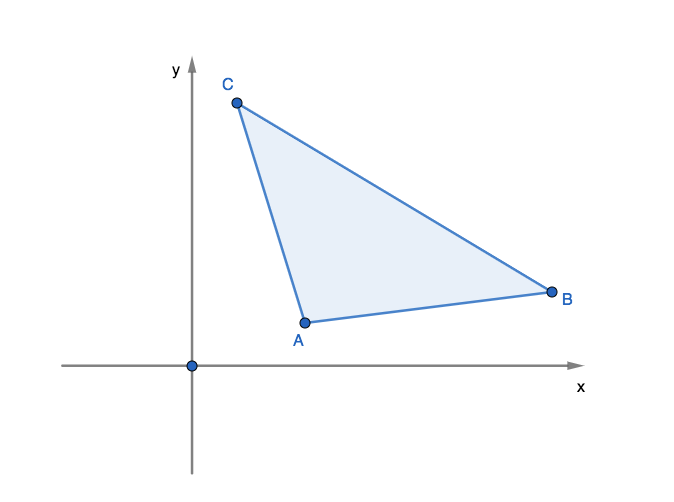
\includegraphics[width=0.8\linewidth]{images/triangle}}
\caption{Произвольный треугольник в двумерной области.}
\label{img:integrate:triangle}
\end{figure}

Барицентрическая система координат представляет собой систему координат, в которой расположение точки симплекса определяется как центр массы или барицентр, как правило, неравных масс, размещенных в его вершинах. 

Мы можем записать декартовы координаты точки $\mathbf{r}$ через декартовы компоненты треугольных вершин $\mathbf{r}_1, \mathbf{r}_2, \mathbf{r}_3$ где $\mathbf{r}_i = (x_i, y_i)$, и в терминах барицентрической системы координат переход будет выглядеть следующим образом:

\begin{eqnarray}
x = \lambda_{1} x_{1} +  \lambda_{2} x_{2} +  \lambda_{3} x_{3} \\
y = \lambda_{1} y_{1} +  \lambda_{2} y_{2} +  \lambda_{3} y_{3} \\
\lambda_{3} = 1 - \lambda_{1} - \lambda_{2}
\end{eqnarray}

Вычисление двойного интеграла в барицентрических координатах осуществляется посредством следующей формулы\cite{bib:calc:barycentric}:

\begin{equation}
\int\limits_{\Delta} f(\mathbf{r}) \ d\mathbf{r} = 2S_{\Delta} \int\limits_{0}^{1} \int\limits_{0}^{1 - \lambda_{2}} f(\lambda_{1} \mathbf{r}_{1} + \lambda_{2} \mathbf{r}_{2} +
(1 - \lambda_{1} - \lambda_{2}) \mathbf{r}_{3}) \ d\lambda_{1} \ d\lambda_{2}
\end{equation}

\subsection{Уравнения мелкой воды в терминах МКЭ}

В рассматриваемой системе \ref{eq:task:1}-\ref{eq:task:2} можно пренебречь членами $-fq_{1}$ и $fq_2$, так как коэффициент Кориолиса очень мал, а также конвективными членами. После отбрасывания неучитываемых членов в \ref{eq:task:1}-\ref{eq:task:2} можно перейти к конечно-элементой формулировке. Для этого необходимо представить функции $q_1(x_1, x_2,t) , q_2(x_1, x_2,t), H(x_1, x_2,t)$ как разложения:

\begin{eqnarray}\label{eq:fem:approx}
q_1(x_1, x_2, t) = \sum\limits_{m=1}^{M} a_m(t)N_m(x, y) \\
q_2(x_1, x_2, t) = \sum\limits_{m=1}^{M} a_{m+k}(t)N_m(x, y) \\
H(x_1, x_2, t) = \sum\limits_{m=1}^{M} a_{2\cdot m+k}(t)N_m(x, y)
\end{eqnarray}

Важно заметить, что в данных разложениях применяются одни и те же весовые функции $N_k$.

Следующим шагом необходимо подставить полученные разложения в исходную систему уравнений. После этого каждое из уравнений необходимо умножить на весовую функцию $W_l(x_1, x_2)$ и проинтегрировать во треугольнику. Также каждое из уравнений необходимо разрешить относительно производной, чтобы получить систему обыкновенных дифференциальных уравнений\cite{bib:calc:gurevich:2004} вида:

\begin{eqnarray}
A \cdot \frac{da}{dt} + B \cdot a + \cdots = f.
\end{eqnarray}

Важно заметить, что каждое из трех исходных уравнений в частных производных дало по $M$ обыкновенных дифференциальных уравнений, и в конечном итоге задача сводится к решению системы из $3\cdot M$ дифференциальных уравнений.

В данной бакалаврской работе конечная система уравнений не была получена аналитически, так как для упрощения решения и минимизации ошибок был использован программный пакет sympy\cite{bib:python:mastering:2015}. С помощью его и системы Jupiter Notebook три формулы для $q_1$, $q_2$ и $H$ соответсвенно  были выведены, а далее запрограммированы с помощью функции solve ivp из пакета scipy и приведены в приложении В.

\chapter{Решение задачи}

\section{Построение графиков}

Для того чтобы визуализировать результаты численных экспериментов, была написана функция, которая строит графики для $q_1$, $q_2$ и $H$ в различные моменты времени. Для лучшей визуализации был написан алгоритм, который комбинирует данные графики в GIF анимацию. Так как количество графиков для некоторых из примеров было достаточно велико, то для создания анимации в случае некоторых экспериментов пришлось писать данные в буфер обмена напрямую, так как в противном случае происходило переполнение и программа переставала работать.

Все графики строятся по изначальным точкам разбиения области. Для того чтобы получить более детальную картинку, была произведена кубическая интерполяция.

Для получения дополнительной информации об эксперименте была написана функция для визуализации графика функции тока:

$$\Psi = \int q_1(x_1, x_2) dx_2$$

Визуализация данной функции дает лучшее понимание о том, каким именно образом распространяются волны в водоеме. Для данных графиков тоже была произведена кубическая интерполяция.

\section{Изменение формы водоёма}

Для программной реализации триангулирования произвольной области был использован Python модуль triangle\cite{bib:website:quake:triangle}, который реализует триангуляцию как с помощью алгоритма Рапперта, так и с помощью алгоритма Чу.

Данный модуль получает на вход геометрию в формате POLY и возвращает список вершин, сегментов, пустых областей, треугольников, маркеров вершин и маркеров сегментов, которые представляют собой нерегулярную сетку для исходной области. Для структуризации этой информации была написана своя реализация для объекта <<точка>> и <<треугольник>>. Экземпляр класса <<точка>> хранит в себе координаты $(x, y)$ и номер точки. Экземпляр класса <<треугольник>> хранит в себе список из трех точек, а также имеет методы для вычисления площади, базисных функций и интегрирования по данному треугольнику. Таким образом, в реализации результат триангуляции представляет из себя массив экземпляров класса <<треугольник>>.

\subsection{Пруд}

В качестве самой простой геометрии был выбран квадратный пруд, в соответсвии с рисунком \ref{img:ex1:contour}.

\begin{figure}[H]
\centerline{
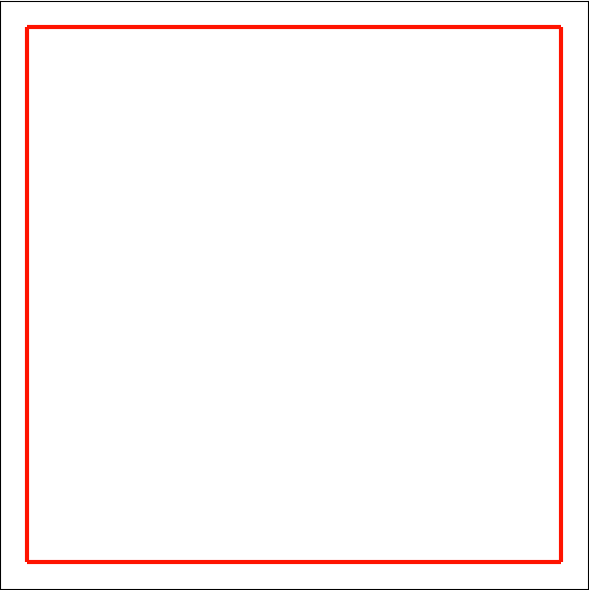
\includegraphics[width=0.5\linewidth]{images/ex1/contour}}
\caption{Квадратный пруд.}
\label{img:ex1:contour}
\end{figure}

Для него было построено разбиение в соответствии с рисунком \ref{img:ex1:mesh}.

\begin{figure}[H]
\centerline{
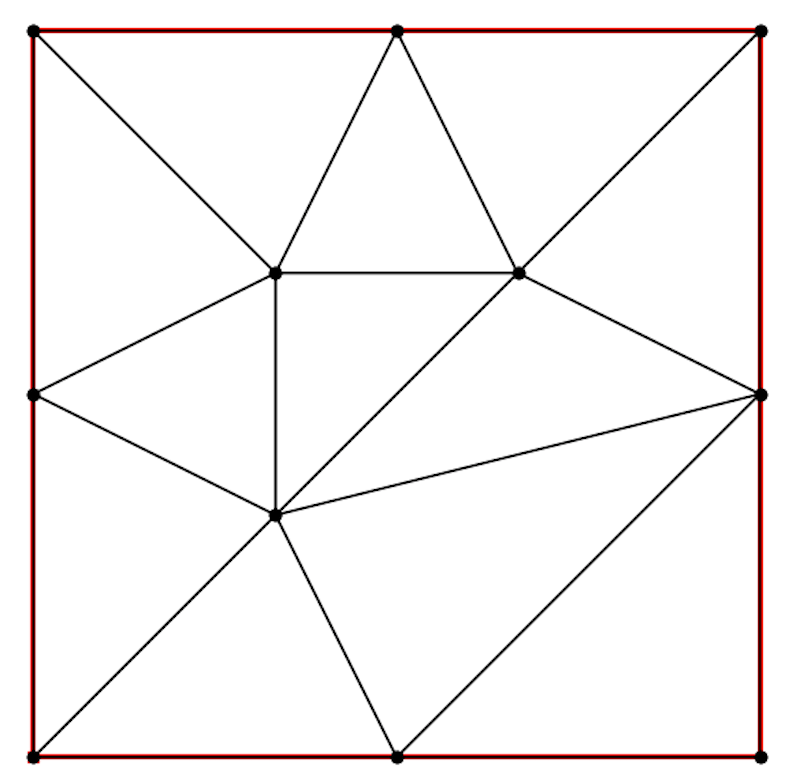
\includegraphics[width=0.5\linewidth]{images/ex1/mesh}}
\caption{Триангуляция квадратного пруда.}
\label{img:ex1:mesh}
\end{figure}


Данный пример рассматривался в моменты времени $0$с, $1$с и $2$с. Для этих моментов времени были получены графики \ref{img:ex1:q1:all}-\ref{img:ex1:psi:all}.

\begin{figure}[H]
  \centering
  \subfloat{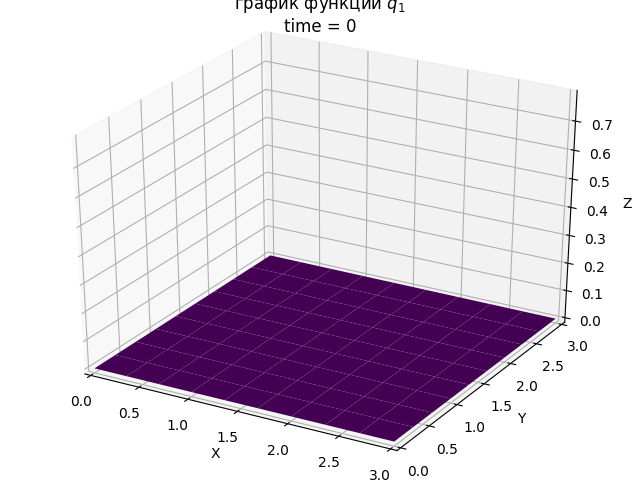
\includegraphics[width=0.39\textwidth]{images/ex1/q_1/0}\label{img:ex1:q1:0}}
  \hfill
  \subfloat{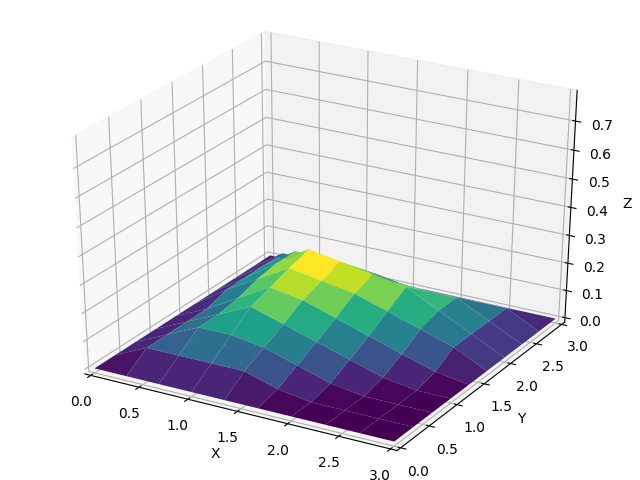
\includegraphics[width=0.39\textwidth]{images/ex1/q_1/1}\label{img:ex1:q1:1}}
  \hfill
  \subfloat{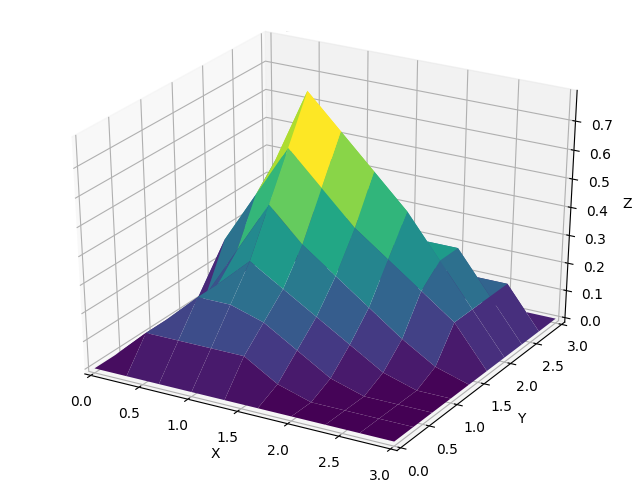
\includegraphics[width=0.39\textwidth]{images/ex1/q_1/2}\label{img:ex1:q1:2}}
  \caption{Изменение проекции потока жидкости на ось $x_1$ в различные промежутки времени.}
  \label{img:ex1:q1:all}
\end{figure}

\begin{figure}[H]
  \centering
  \subfloat{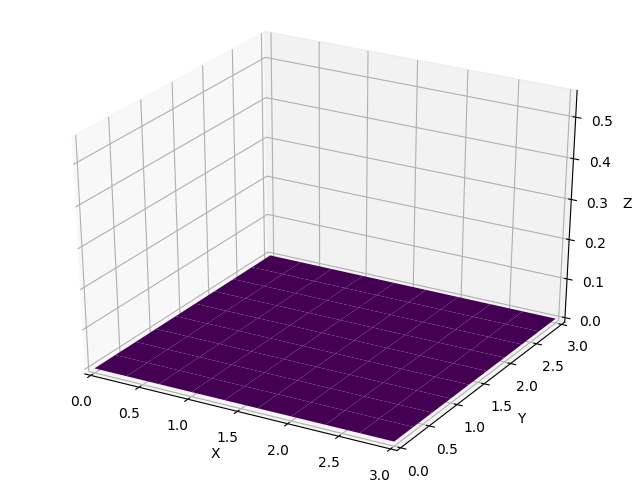
\includegraphics[width=0.39\textwidth]{images/ex1/q_2/0}\label{img:ex1:q2:0}}
  \hfill
  \subfloat{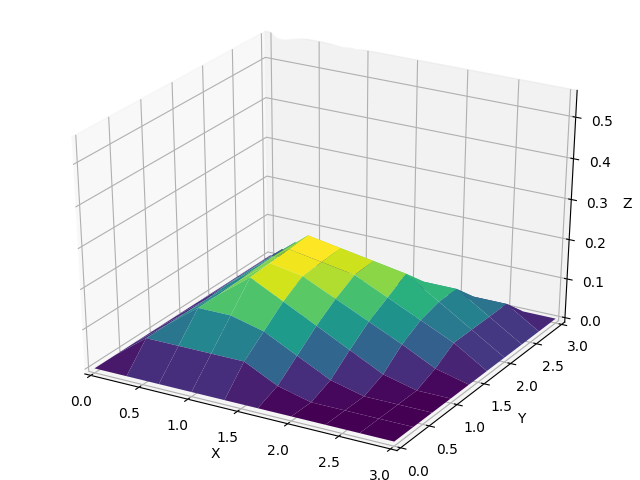
\includegraphics[width=0.39\textwidth]{images/ex1/q_2/1}\label{img:ex1:q2:1}}
  \hfill
  \subfloat{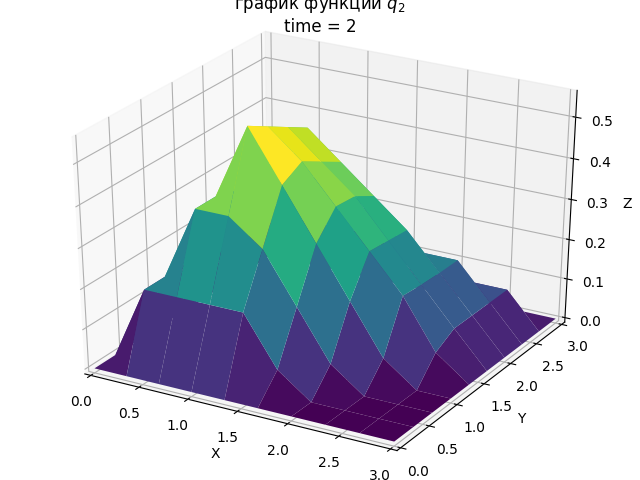
\includegraphics[width=0.39\textwidth]{images/ex1/q_2/2}\label{img:ex1:q2:2}}
  \caption{Изменение проекции потока жидкости на ось $x_2$ в различные промежутки времени.}
  \label{img:ex1:q2:all}
\end{figure}

\begin{figure}[H]
  \centering
  \subfloat{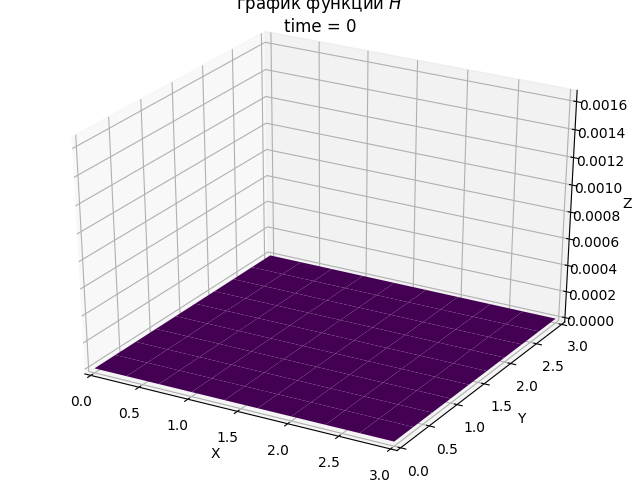
\includegraphics[width=0.39\textwidth]{images/ex1/H/0}\label{images/ex1/H/0}}
  \hfill
  \subfloat{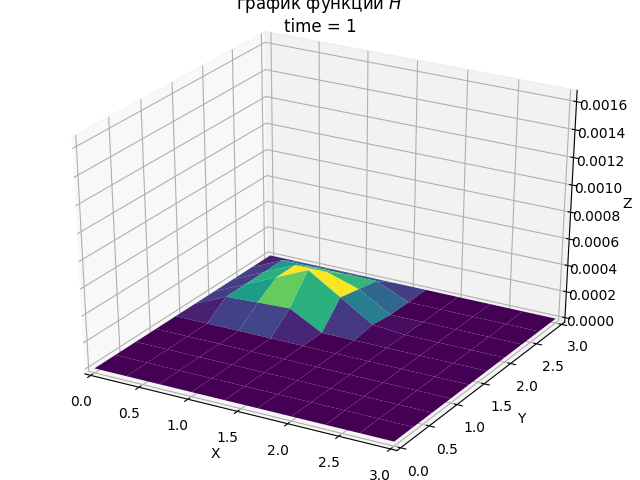
\includegraphics[width=0.39\textwidth]{images/ex1/H/1}\label{images/ex1/H/1}}
    \hfill
  \subfloat{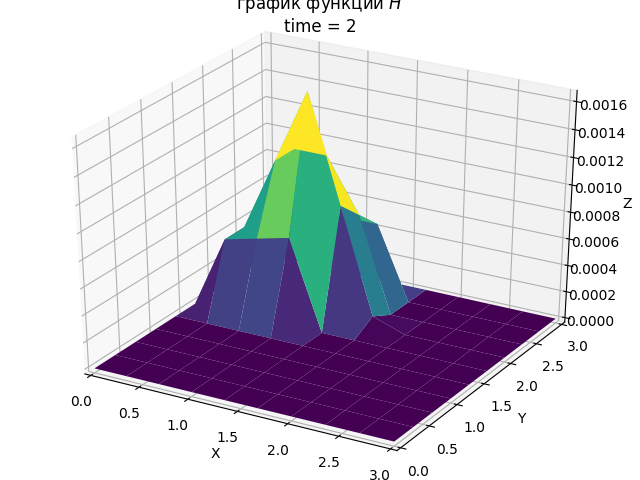
\includegraphics[width=0.39\textwidth]{images/ex1/H/2}\label{img:ex1:H:2}}
  \caption{Изменение высоты в различные промежутки времени.}
  \label{img:ex1:H:all}
\end{figure}


\begin{figure}[H]
  \centering
  \subfloat{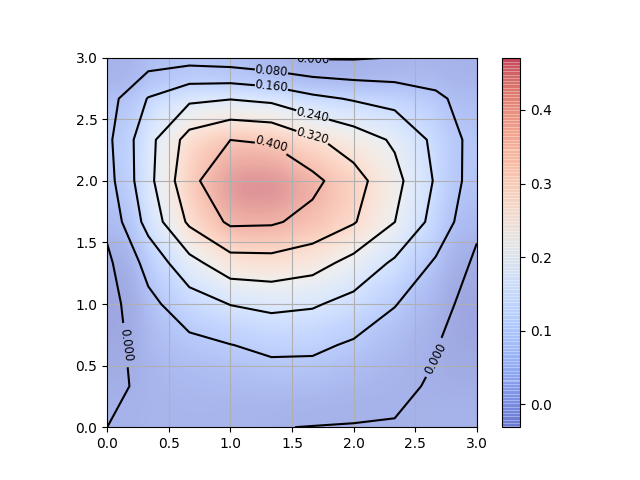
\includegraphics[width=0.425\textwidth]{images/ex1/psi/1}\label{img:ex1:psi:1}}
    \hfill
  \subfloat{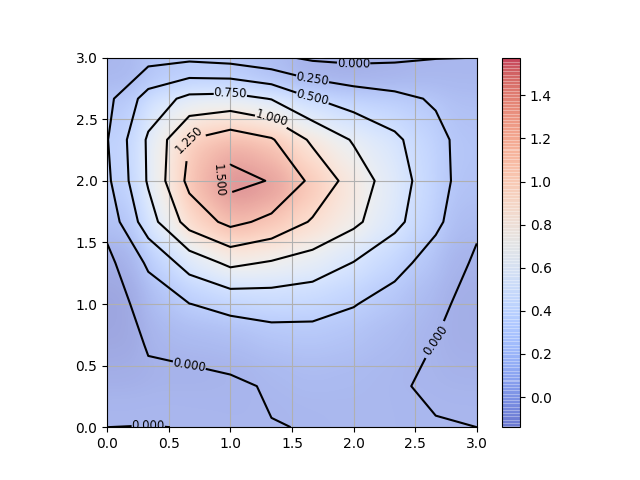
\includegraphics[width=0.425\textwidth]{images/ex1/psi/2}\label{img:ex1:psi:2}}
  \caption{Изменение функции тока в различные промежутки времени.}
  \label{img:ex1:psi:all}
\end{figure}


\subsection{Реальный водоём}


В качестве реального водоема, у которого нет островов, было выбрано озеро Эльтон -- солёное бессточное самосадочное озеро на севере Прикаспийской низменности, изображенное на рисунке \ref{img:lake:elton}. Данное озеро имеет площадь в $152$ квадратных километра и наибольшую глубину до $1.5$ метров. В среднем глубина данного озера составляет $0.05 - 0.07$ метра, а это значит, что для данного озера будут справедливыми уравнения мелкой воды.

\begin{figure}[H]
\centerline{
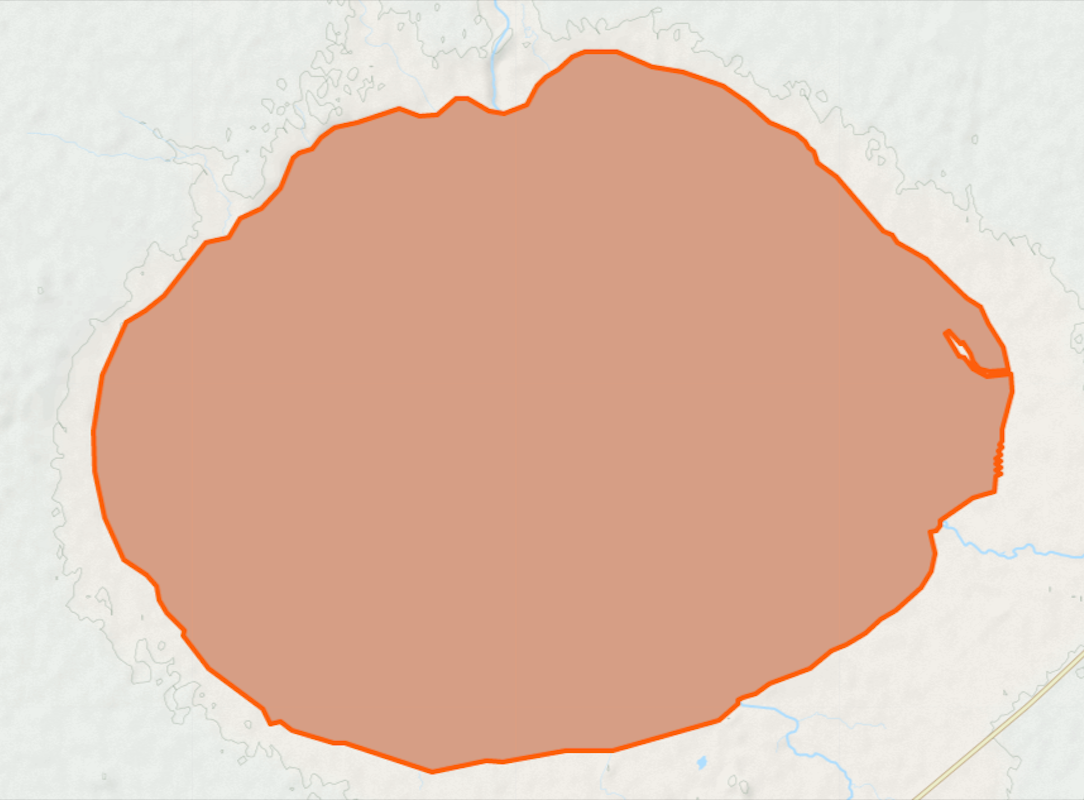
\includegraphics[width=0.6\linewidth]{images/ex2/lake_elton}}
\caption{Озеро Эльтон, выделенное на карте OSM.}
\label{img:lake:elton}
\end{figure}

Данные для расчета задачи по озеру Эльтон были получены на основании системы OSM\cite{bib:website:osm} -- некоммерческого веб-картографического проекта. Для этого был использован сервис overpass-turbo\cite{bib:website:overpassturbo}, который является интерфейсом к API OSM и позволяет очень просто выполнять необходимые запросы. Запрос для озера Эльтон выглядит следующим образом:

\begin{lstlisting}[frame=single]
[out:json][timeout:25];
(
  node["name"="Elton"]({{bbox}});
  way["name"="Elton"]({{bbox}});
  relation["name"="Elton"]({{bbox}});
);
out body;
>;
out skel qt;	
\end{lstlisting}

Одним из результатов запроса будет $geojson$ файл, в котором содержатся точки запрашиваемого географического объекта и некоторая метаинформация. Так как для триангуляции требуется файл с геометрией в формате POLY, то была написана соответствующая функция на языке $Python$, которая конвертирует формат $geojson$ в формат POLY. Для озера Эльтон было построено разбиение в соответствии с рисунком \ref{img:ex2:mesh}.

\begin{figure}[H]
\centerline{
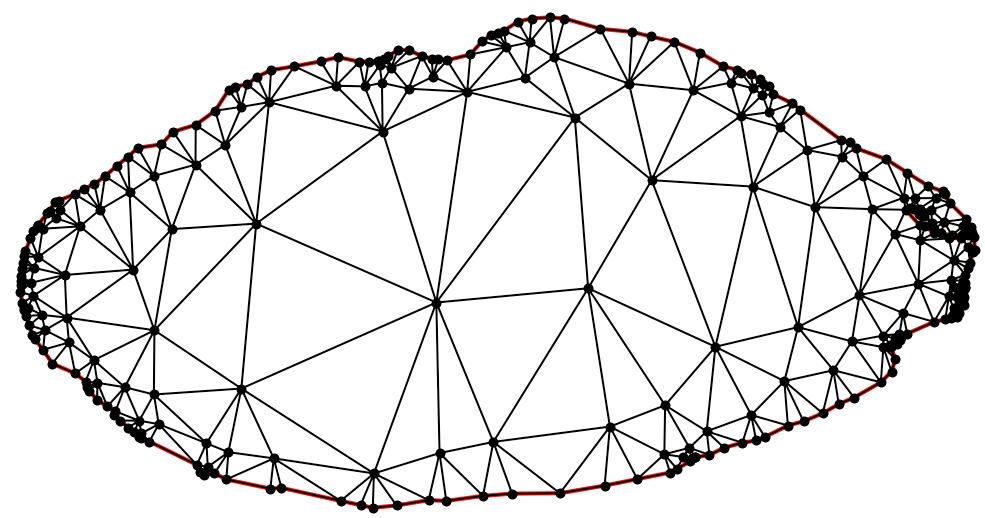
\includegraphics[width=1.0\linewidth]{images/ex2/mesh}}
\caption{Триангуляция озера Эльтон.}
\label{img:ex2:mesh}
\end{figure}

Данный пример рассматривался в моментах времени $1.902$с и $1.905$с. Для этих моментов времени были получены графики \ref{img:ex2:q1:all}-\ref{img:ex2:psi:all}.

\begin{figure}[H]
  \centering
  \subfloat{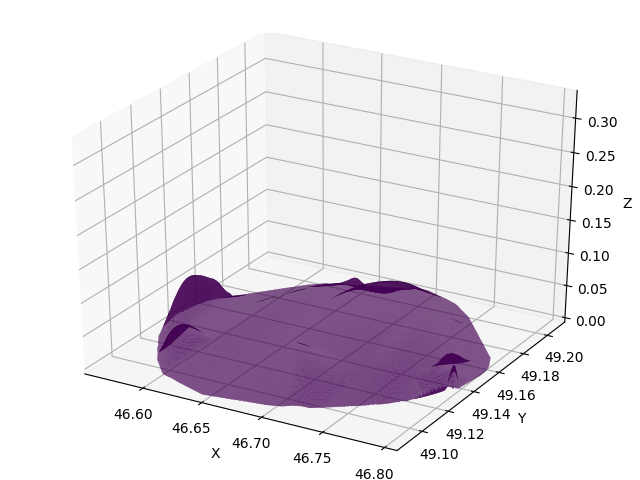
\includegraphics[width=0.425\textwidth]{images/ex2/q_1/902}\label{img:ex2:q1:902}}
  \hfill
  \subfloat{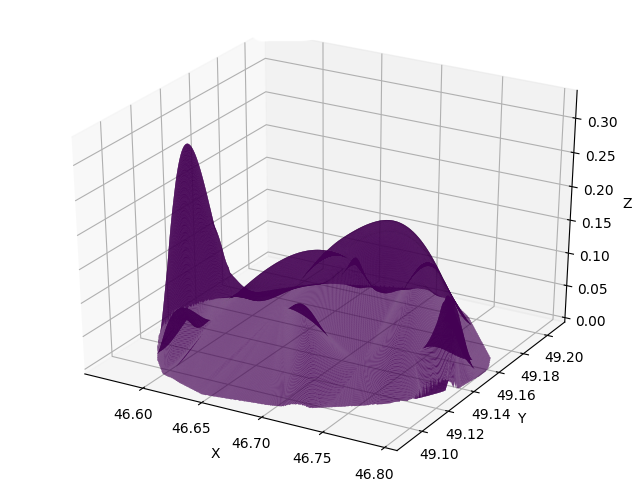
\includegraphics[width=0.425\textwidth]{images/ex2/q_1/905}\label{img:ex2:q1:905}}
  \caption{Изменение проекции потока жидкости на ось $x_1$ в различные промежутки времени.}
  \label{img:ex2:q1:all}
\end{figure}

\begin{figure}[H]
  \centering
  \subfloat{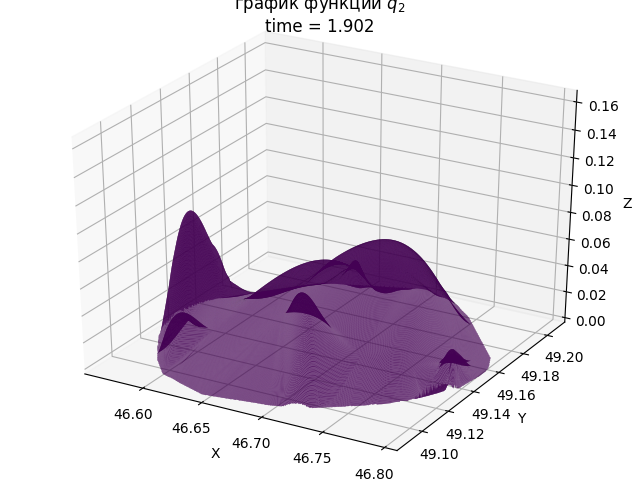
\includegraphics[width=0.425\textwidth]{images/ex2/q_2/902}\label{img:ex2:q2:902}}
  \hfill
  \subfloat{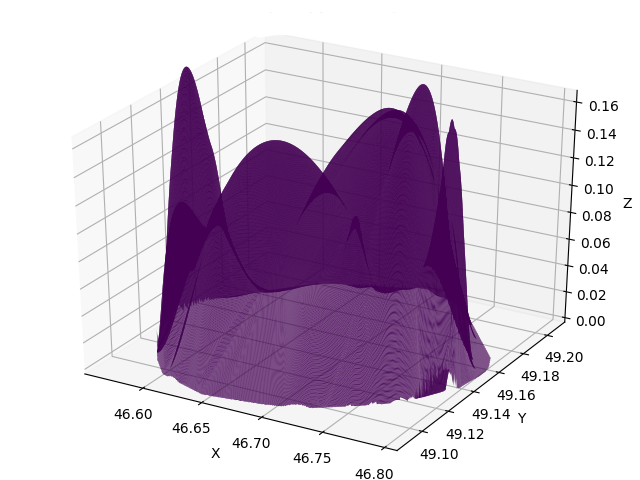
\includegraphics[width=0.425\textwidth]{images/ex2/q_2/905}\label{img:ex2:q2:905}}
  \caption{Изменение проекции потока жидкости на ось $x_2$ в различные промежутки времени.}
  \label{img:ex2:q2:all}
\end{figure}

\begin{figure}[H]
  \centering
  \subfloat{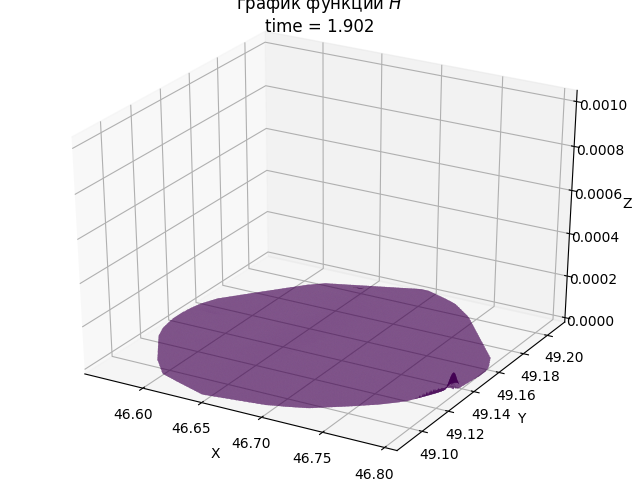
\includegraphics[width=0.425\textwidth]{images/ex2/H/902}\label{images/ex2/H/902}}
  \hfill
  \subfloat{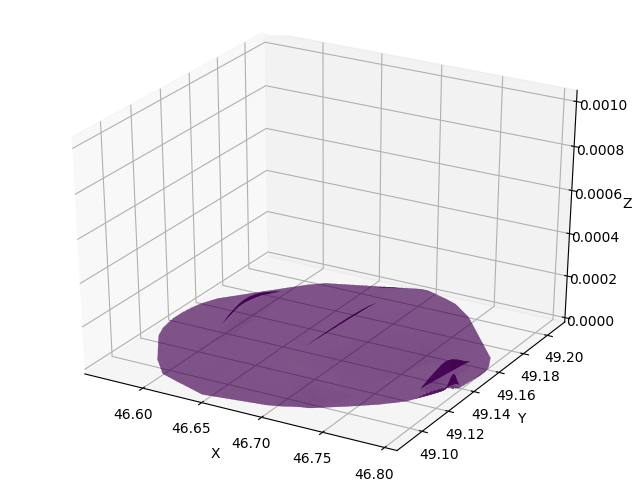
\includegraphics[width=0.425\textwidth]{images/ex2/H/905}\label{images/ex2/H/905}}
  \caption{Изменение высоты в различные промежутки времени.}
  \label{img:ex2:H:all}
\end{figure}

\begin{figure}[H]
  \centering
  \subfloat{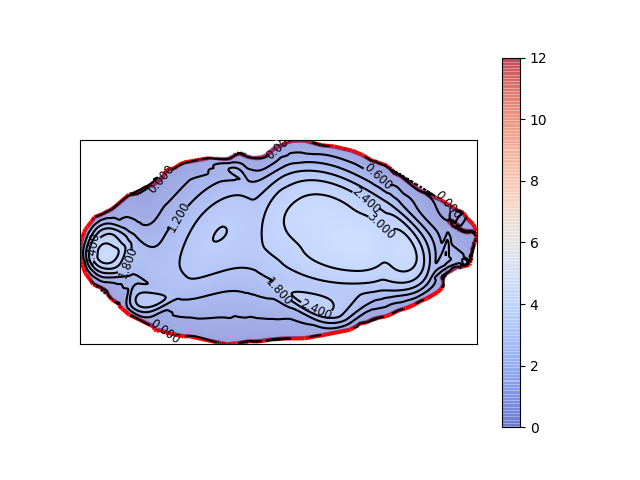
\includegraphics[width=0.425\textwidth]{images/ex2/psi/902}\label{images/ex2/psi/902}}
  \hfill
  \subfloat{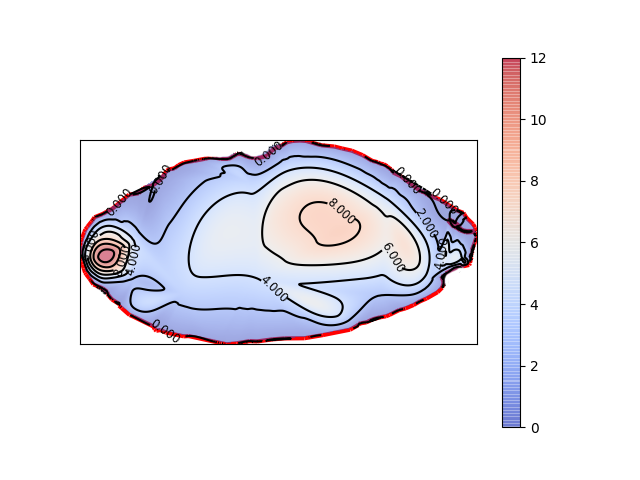
\includegraphics[width=0.425\textwidth]{images/ex2/psi/905}\label{images/ex2/psi/905}}
  \caption{Изменение функции тока в различные промежутки времени.}
  \label{img:ex2:psi:all}
\end{figure}

\section{Учёт наличия острова (островов) внутри водоёма}

\subsection{Пруд}
Для того чтобы проверить корректность алгоритма на сетках с <<дырами>>, в пруд, рассмотренный ранее, добавлено два острова, в соответсвии с рисунком \ref{img:ex3:contour}.

\begin{figure}[H]
\centerline{
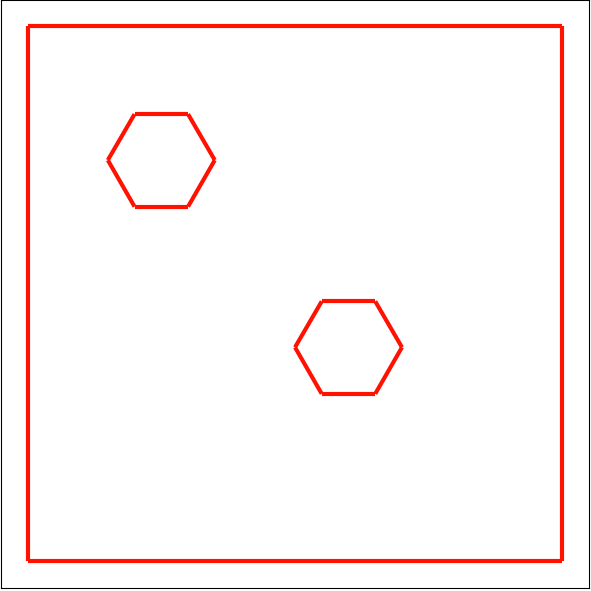
\includegraphics[width=0.5\linewidth]{images/ex3/contour}}
\caption{Квадратный пруд с двумя островами.}
\label{img:ex3:contour}
\end{figure}

Для этой геометрии было построено разбиение в соответствии с рисунком \ref{img:ex3:mesh}.

\begin{figure}[H]
\centerline{
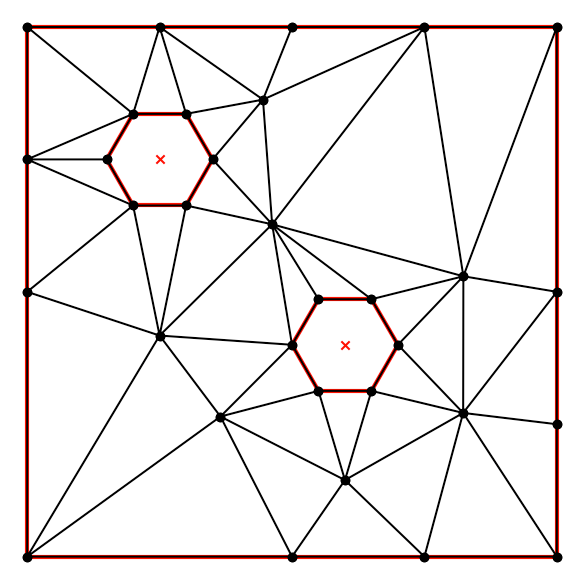
\includegraphics[width=0.5\linewidth]{images/ex3/mesh}}
\caption{Триангуляция прямоугольного пруда с двумя островами.}
\label{img:ex3:mesh}
\end{figure}

Данный пример рассматривался на двух моментах времени: $1.91$с и $1.99$с. Для этих моментов времени были получены графики \ref{img:ex1:q1:all}-\ref{img:ex3:psi:all}.

\begin{figure}[H]
  \centering
  \subfloat{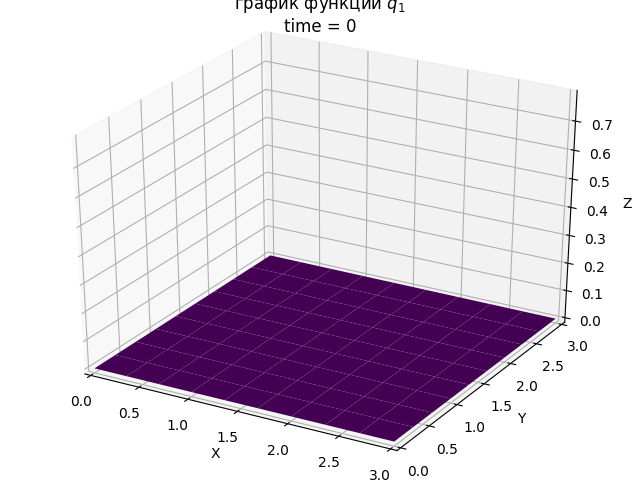
\includegraphics[width=0.39\textwidth]{images/ex1/q_1/0}\label{img:ex3:q1:91}}
  \hfill
  \subfloat{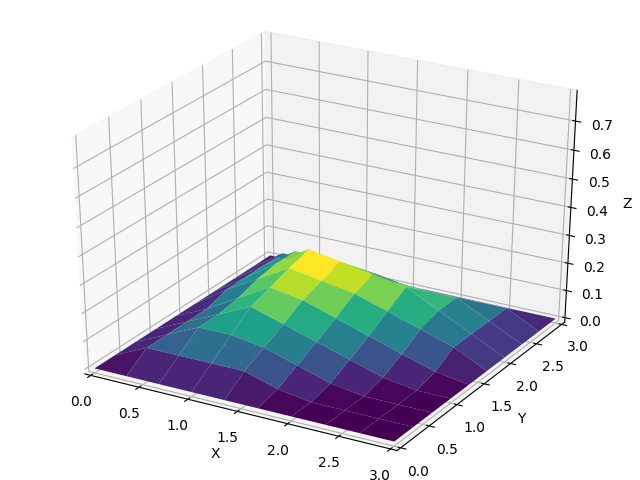
\includegraphics[width=0.39\textwidth]{images/ex1/q_1/1}\label{img:ex3:q1:99}}
  \caption{Изменение проекции потока жидкости на ось $x_1$ в различные промежутки времени.}
  \label{img:ex3:q1:all}
\end{figure}

\begin{figure}[H]
  \centering
  \subfloat{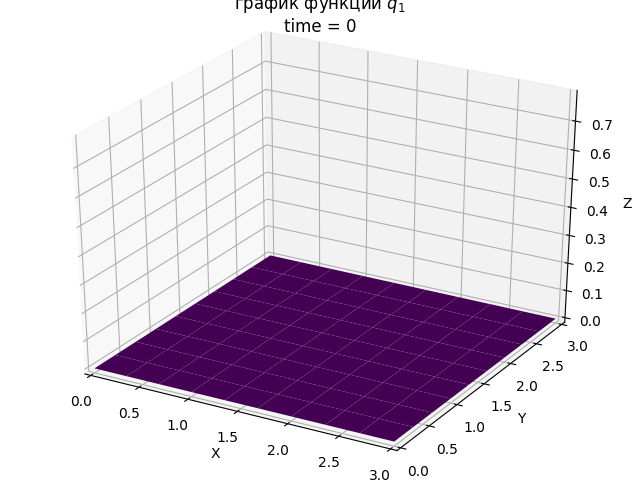
\includegraphics[width=0.39\textwidth]{images/ex1/q_1/0}\label{img:ex3:q2:91}}
  \hfill
  \subfloat{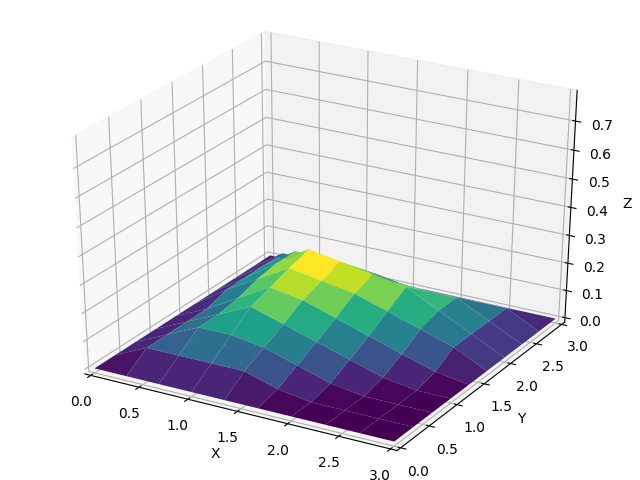
\includegraphics[width=0.39\textwidth]{images/ex1/q_1/1}\label{img:ex3:q2:99}}
  \caption{Изменение проекции потока жидкости на ось $x_2$ в различные промежутки времени.}
  \label{img:ex3:q2:all}
\end{figure}

\begin{figure}[H]
  \centering
  \subfloat{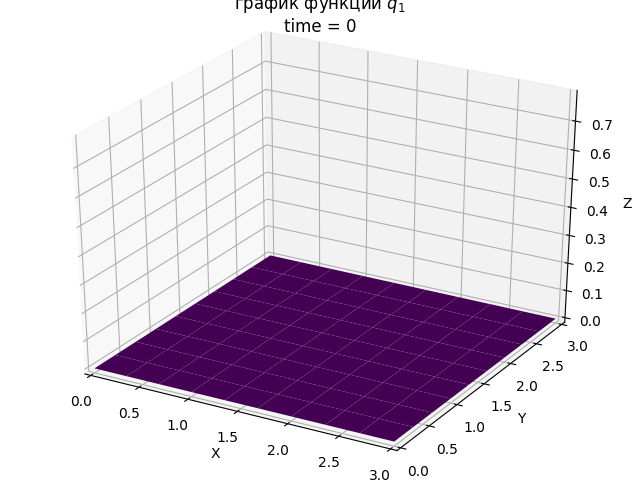
\includegraphics[width=0.39\textwidth]{images/ex1/q_1/0}\label{img:ex3:H:91}}
  \hfill
  \subfloat{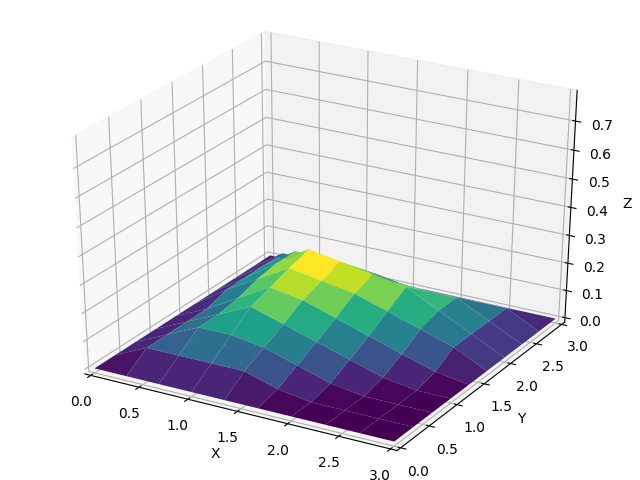
\includegraphics[width=0.39\textwidth]{images/ex1/q_1/1}\label{img:ex3:H:99}}
  \caption{Изменение высоты в различные промежутки времени.}
  \label{img:ex3:H:all}
\end{figure}

\begin{figure}[H]
  \centering
  \subfloat{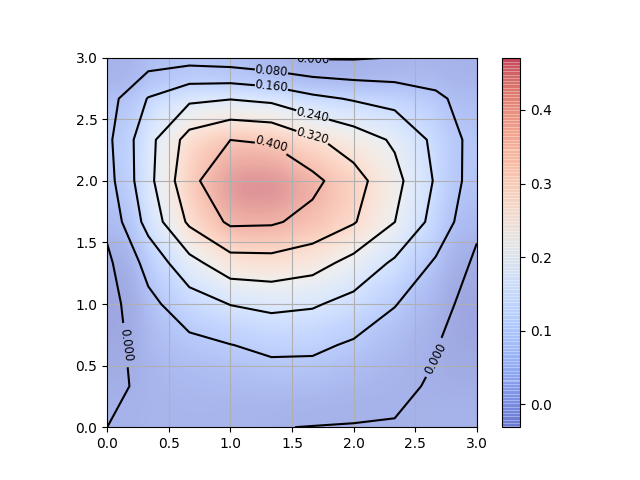
\includegraphics[width=0.425\textwidth]{images/ex1/psi/1}\label{img:ex3:psi:91}}
    \hfill
  \subfloat{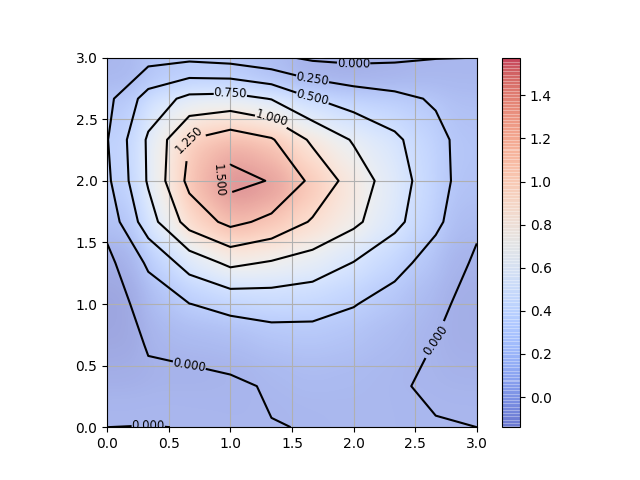
\includegraphics[width=0.425\textwidth]{images/ex1/psi/2}\label{img:ex3:psi:99}}
  \caption{Изменение функции тока в различные промежутки времени.}
  \label{img:ex3:psi:all}
\end{figure}

\subsection{Реальный водоём}
В качестве реального водоема, у которого есть острова, было выбрано озеро Верхнее, изображенное на рисунке \ref{img:lake:superior}. Оно находится в Северной Америке и является самым крупным и глубоким в системе Великих озёр. С физической точки зрения глубина этого озера составляет максимум 406 метров, а его размеры -- 563 x 257 км. Получается, что для него можно использовать уравнения мелкой воды.

\begin{figure}[H]
\centerline{
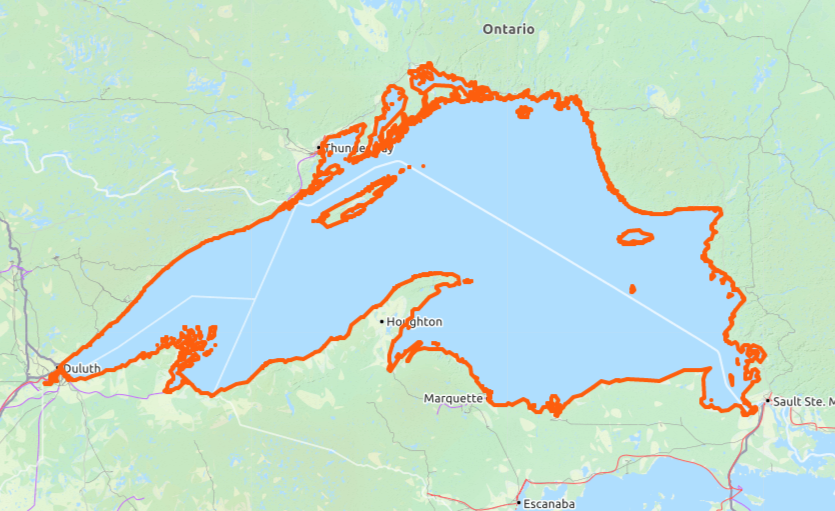
\includegraphics[width=0.8\linewidth]{images/ex4/lake_superior}}
\caption{Озеро Верхнее выделенное на карте OSM.}
\label{img:lake:superior}
\end{figure}

Для этой геометрии было построено разбиение в соответствии с рисунком \ref{img:ex4:mesh}.

\begin{figure}[H]
\centerline{
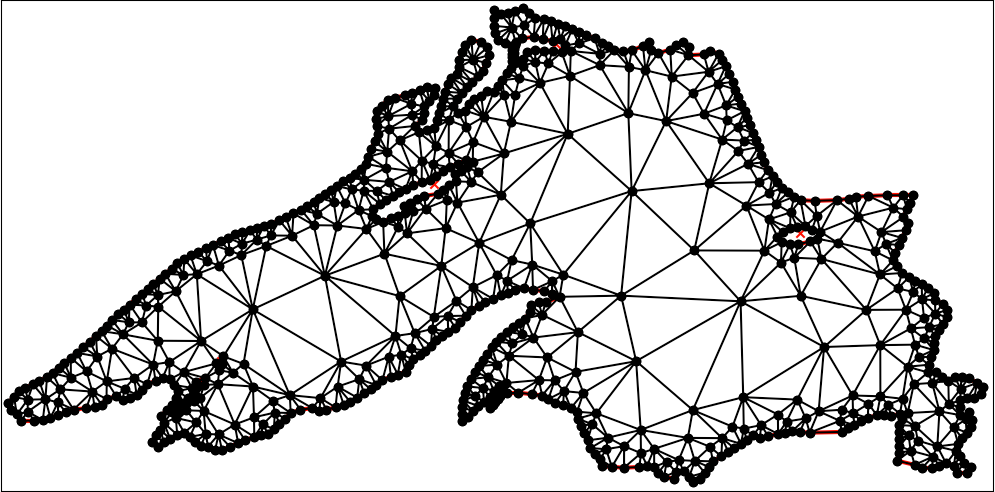
\includegraphics[width=0.8\linewidth]{images/ex4/mesh}}
\caption{Триангуляция озера Верхнее.}
\label{img:ex4:mesh}
\end{figure}

Для озера Верхнее были произведены расчеты аналогичные расчетам для пруда и построен график функции тока для качественной оценки движения волн, который изображен на рисунке \ref{img:ex4:psi}.

\begin{figure}[H]
\centerline{
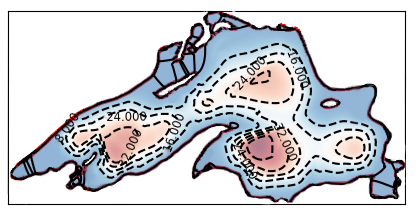
\includegraphics[width=0.8\linewidth]{images/ex4/psi/1}}
\caption{График функции тока.}
\label{img:ex4:psi}
\end{figure}


\section{Программная реализация}

МКЭ является очень ресурсоемким методом, и именно из-за этого он долго не применялся. Все современные задачи считаются на больших сетках, и занимает это достаточно большое количество времени.

Именно по этой причине реализация МКЭ в данной бакалаврской работе является многопоточной. В первую очередь это удалось сделать благодаря самому МКЭ, который позволяет считать элементы в сетке независимо друг от друга. 

Для решения этой задачи был написан пулл потоков, который позволяет в один и тот же момент времени считать произвольное количество элементов, которое варьируется от 1 до $n$, где $n$ -- максимально возможное количество потоков, которое может одновременно исполнять компьютер на котором запущенна программа.

Так как при использовании потоков Python не может задействовать все ядра процессора для выполнения нескольких потоков одновременно, то вместо них в реализации задачи были использованы процессы из библиотеки multiprocessing.

Помимо этого все модули приложения вместе с внешними зависимостями были упакованы в Docker контейнер, который позволяет очень просто переносить приложение на любую систему, которая поддерживает данную технологию. Данная упаковка позволила производить вычисления не на личном стационарном компьютере, а на удаленном сервере, который имеет намного большие вычислительные мощности и позволяет быстрее получить результат.

\chapter{Разработка базы данных для хранения информации о проведённых экспериментах}

Данные, полученные в результате численных экспериментов, являются разрозненными, так как они представляют из себя не только GIF анимацию, но и некоторую метаинформацию, которая представлена в виде JSON файлов. Из-за этого, помимо общепринятых требований к БД, следует основываясь на приведенной выше специфике данных, которые были получены в результате решения поставленной задачи, ввести следующие требования, которым должны удовлетворять БД и СУБД, управляющая ей:

\begin{enumerate}

\item Запись об эксперименте должна позволять хранить любую метаинформацию, которая может различаться в зависимости от проведенного эксперимента

\item БД должна позволять добавлять поля к уже существующим данным. Это, к примеру, нужно для добавления в запись данных, которые получены в результате постобработки эксперимента человеком

\item БД должна легко масштабироваться, так как данных может быть много

\item Должно быть отсутствие необходимости сопоставления объекта в базе и программе для упрощения разработки

\item Хранение графической информации должно быть реализовано максимально просто и эффективно

\end{enumerate}

\section{Описание базы данных}

Основываясь на приведенных выше требованиях, в качестве СУБД решено выбрать MongoDB, которая классифицируется как NoSQL. MongoDB — документо-ориентированная система управления базами данных с открытым исходным кодом, не требующая описания схемы таблиц. Каждая запись – это документ без жёстко заданной схемы, который может содержать вложенные документы.

Так как документо-ориентированные базы данных еще не так распространены, как реляционные, но их популярность с каждым годом все увеличивается, целесообразно будет разъяснить некоторые нюансы терминологии документо-ориентированных баз данных. 

В книге о MongoDB\cite{bib:mongo} приведены шесть основных концепций MongoDB:

\begin{enumerate}

\item MongoDB концептуально является тем же самым, что и привычная нам база данных (в терминологии Oracle RDBMS -- схема). Внутри MongoDB может быть ноль или более баз данных, каждая из которых является контейнером для прочих сущностей.

\item База данных может иметь ноль или более <<коллекций>>. <<Коллекция>> настолько похожа на традиционную <<таблицу>>, что можно смело считать их одним и тем же.

\item <<Коллекции>> состоят из нуля или более <<документов>>, каждый из которых можно рассматривать как <<строку>>.

\item <<Документ>> состоит из одного или более <<полей>>, которые подобны <<колонкам>>.

\item <<Индексы>> в MongoDB почти идентичны таковым в реляционных базах данных.

\item <<Курсоры>> отличаются от предыдущих пяти концепций, но они очень важны. Когда мы запрашиваем у MongoDB какие-либо данные, то БД возвращает <<курсор>>, с которым мы можем делать все что угодно: подсчитывать, пропускать определённое число предшествующих записей, - при этом не загружая сами данные.

\end{enumerate}

Если резюмировать сказанное выше, то MongoDB состоит из <<баз данных>>, которые, в свою очередь, состоят из <<коллекций>>. <<Коллекции>> состоят из <<документов>>, а каждый <<документ>> - из <<полей>>. <<Коллекции>> могут быть проиндексированы, что улучшает производительность выборки и сортировки. И наконец, получение данных из MongoDB сводится к получению <<курсора>>, который отдаёт эти данные по мере надобности.

Также стоит привести основные достоинства данной базы данных:

\begin{enumerate}

\item Документо-ориентированное хранилище (простая и мощная JSON-подобная схема данных)
\item Достаточно гибкий язык для формирования запросов
\item Динамические запросы
\item Полная поддержка индексов
\item Профилирование запросов
\item Эффективное хранение двоичных данных больших объёмов, например фото и видео
\item Журналирование операций, модифицирующих данные в БД
\item Поддержка отказоустойчивости и масштабируемости: асинхронная репликация, набор реплик и шардинг

\end{enumerate}

Основными плюсами MongoDB, помимо её документо-ориентированности, для данной бакаларвской работы стали:

\begin{enumerate}

\item Схожий с реляционными СУБД подход к хранению данных, который построен на следующем: база данных-коллекция-документ-поле

\item Формат хранения данных. Данные в MongoDB хранятся в формате BSON. BSON - это бинарный формат, используемый для хранения документов и осуществления удаленного вызова процедур в MongoDB. Тот факт, что данные хранятся именно в бинарном виде, значительно ускоряет время их автоматической обработки

\item Простота разработки. MongoDB, в отличии от конкурентов, достаточно просто разворачивается и администрируется, а также имеет хороший API 

\item GridFS -- файловая система, которая поставляется вместе с MongoDB и служит для хранения больших файлов

\end{enumerate}


\section{Формат представления данных в БД}

Так как в качестве СУБД была выбрана документо-ориентированная MongoDB, то и структура базы данных будет приводится в её терминологии. 

Основной и единственной базой данных является база <<эксперименты>> (<<experiments>>). В ней находится коллекция  <<данные>> (<<data>>). Данная коллекция содержит в себе документы, каждый из которых является проведенным экспериментов. Структура базы данных изображена на рисунке \ref{img:database}.

\begin{figure}[H]
\centerline{
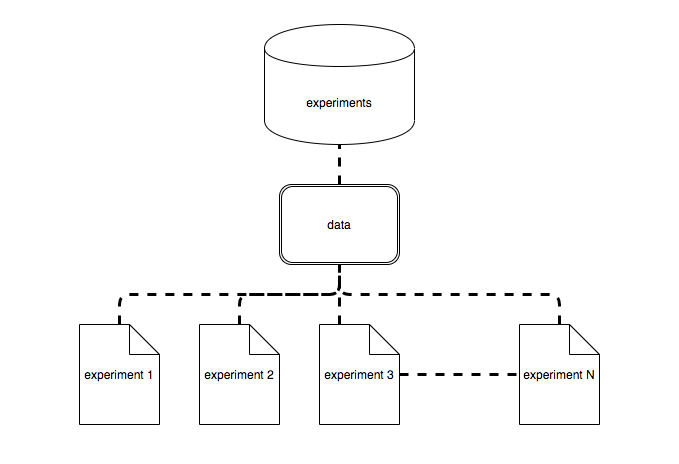
\includegraphics[width=1.0\linewidth]{images/database}}
\caption{Структура БД.}
\label{img:database}
\end{figure}

Каждый из содержащихся в БД документов хранит в себе следующие поля:

\begin{enumerate}
\item дата проведения эксперимента
\item время выполнения эксперимента
\item уникальный идентификатор, указывающий на изображения, полученные в результате экспериментов, которые хранятся в GridFS
\item матрица решения системы ОДУ
\item вектор, хранящий в себе моменты времени, в которых была решена ОДУ
\item тип и файл сетки
\item количество базисных функций
\end{enumerate}

Документ, который описывает эксперимент, имеет следующую структуру (в подобном виде он хранится в MongoDB):

\begin{minipage}{\linewidth}
\lstinputlisting{code/json/collection.json}
\end{minipage}

Поля с постфиксами id являются уникальными идентификаторами для GIF анимаций, которые сохранены на файловой системе GridFS. Благодаря этому изображения результатов экспериментов не пропадут в случае отказа одной из нод кластера MongoDB. Таким образом обеспечивается надежная сохранность данных.

\section{Примеры запросов к БД}
Для того чтобы использовать данные, сохраненные в БД в результате экспериментов, можно использовать запросы вида:

\begin{lstlisting}
db.data.find({"date" : "2018-04-24-20-07"})
\end{lstlisting}

Это не очень удобно, так как результатами экспериментов является не только текстовая информация, но еще и графическая. В случае прямого запроса в ответе будут бинарные объекты, с которыми тяжело работать в чистом виде. Именно из-за этого для более простой работы с базой данных была написана функция $save(db, data, dir)$, которая находится в в модуле $fem.db.mongo$. На вход данной функции подается JSON, который является результатом прямого запроса к базе, а также папка, в которую будут сохранены графики эксперимента. Помимо функции $save(db, data, dir)$, в том же пакете находится функция $read(db, collection, date)$, которая позволяет пользователю не делать прямые запросы в базу и облегчает работу с результатами. Комбинированный пример получения данных из базы выглядит следующим образом:

\begin{lstlisting}
save(db, read(db, 'data', '2018-04-24-20-07'), '/data')
\end{lstlisting}

Данный вызов, во-первых, найдет в базе данных документ, в котором хранится информация о результатах эксперимента, который был проведен 2018-04-24-20-07, а во-вторых, сохранит все необходимые результаты на диск в папку /data. Это очень удобно, так как не требует от конечного пользователя знаний о структуре запросов в MongoDB. 


\conclusions

В представленной бакалаврской работе были получены уравнения мелкой воды при пренебрежении температурными эффектами, а также написана многопоточная программная реализация МКЭ для решений данных уравнений.

Реализована возможность переносимости разработанного алгоритма, а также возможность его удаленного использования посредством контейнеризации.

В качестве примера были произведены расчеты на различных сетках, в том числе и на реальных озерах(Эльтон и Верхнее). Для данных расчетов были построены графики на которых изображены изменения потока жидкости и высоты волны, кроме того была сконстурированна функция тока для которой тоже были построены соотвествующие графики. Благодаря данным результатам удалось качественно оценить полученные результаты проведенных экспериментов.

\bibliographystyle{biblio/tst}
\bibliography{biblio/biblio}

\Appendix

\chapter{Исходный код реализации}

Для того, чтобы код можно было легко поддерживать и переиспользовать было произведено разбиение на пакеты и модули в соответсвии с рисунком \ref{img:code:struct}. Основные константы и пути были вынесены в модуль main.py, что позволило очень быстро изменять взодные данные для различных экспериментов.

\begin{figure}[H]
\centerline{
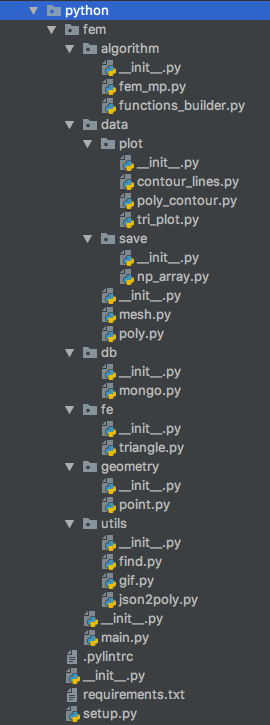
\includegraphics[width=0.4\linewidth]{images/code_struct}}
\caption{Структура пакетов программной реализации метода конечных элементов.}
\label{img:code:struct}
\end{figure}

\lstinputlisting[language=Python, numbers=left, breaklines=true, basicstyle=\scriptsize, caption=Модуль fem\_mp.py]{../python/fem/algorithm/fem_mp.py}

\lstinputlisting[language=Python, numbers=left, breaklines=true, basicstyle=\scriptsize, caption=Модуль functions\_builder.py]{../python/fem/algorithm/functions_builder.py}

\lstinputlisting[language=Python, numbers=left, breaklines=true, basicstyle=\scriptsize, caption=Модуль poly\_contour.py]{../python/fem/data/plot/poly_contour.py}

\lstinputlisting[language=Python, numbers=left, breaklines=true, basicstyle=\scriptsize, caption=Модуль contour\_lines.py]{../python/fem/data/plot/contour_lines.py}

\lstinputlisting[language=Python, numbers=left, breaklines=true, basicstyle=\scriptsize, caption=Модуль tri\_plot.py]{../python/fem/data/plot/tri_plot.py}

\lstinputlisting[language=Python, numbers=left, breaklines=true, basicstyle=\scriptsize, caption=Модуль np\_array.py]{../python/fem/data/save/np_array.py}

\lstinputlisting[language=Python, numbers=left, breaklines=true, basicstyle=\scriptsize, caption=Модуль mesh.py]{../python/fem/data/mesh.py}

\lstinputlisting[language=Python, numbers=left, breaklines=true, basicstyle=\scriptsize, caption=Модуль poly.py]{../python/fem/data/poly.py}

\lstinputlisting[language=Python, numbers=left, breaklines=true, basicstyle=\scriptsize, caption=Модуль mongo.py]{../python/fem/db/mongo.py}

\lstinputlisting[language=Python, numbers=left, breaklines=true, basicstyle=\scriptsize, caption=Модуль triangle.py]{../python/fem/fe/triangle.py}

\lstinputlisting[language=Python, numbers=left, breaklines=true, basicstyle=\scriptsize, caption=Модуль point.py]{../python/fem/geometry/point.py}

\lstinputlisting[language=Python, numbers=left, breaklines=true, basicstyle=\scriptsize, caption=Модуль find.py]{../python/fem/utils/find.py}

\lstinputlisting[language=Python, numbers=left, breaklines=true, basicstyle=\scriptsize, caption=Модуль gif.py]{../python/fem/utils/gif.py}

\lstinputlisting[language=Python, numbers=left, breaklines=true, basicstyle=\scriptsize, caption=Модуль json2poly.py]{../python/fem/utils/json2poly.py}

\lstinputlisting[language=Python, numbers=left, breaklines=true, basicstyle=\scriptsize, caption=Модуль main.py]{../python/fem/main.py}

\chapter{Исходный код Docker контейнера}

Предполагается, что в этой же папке с файлом для сборки контейнера лежит файл requirements.txt, а также исходный код реализации в папке fem и все необходимые ресурсы в папке resources.

\begin{minipage}{\linewidth}
\lstinputlisting[numbers=left, breaklines=true, caption={Dockerfile}]{code/Dockerfile}
\end{minipage}

\begin{minipage}{\linewidth}
\lstinputlisting[numbers=left, breaklines=true, caption={requirements.txt}]{../python/requirements.txt}
\end{minipage}
 
\chapter{Выкладки для МКЭ}

 Для более краткой записи выкладок не будем записывать зависимость весовых функций от $(x_1, x_2)$, а переменных $a_k, a_{m+k}, a_{2m+k}$ от времени $t$.

\section{Уравнение неразрывности}

Запишем исходный вид уравнения:

\begin{eqnarray}
\dfrac{d}{d x_{1}} q_{1} + \dfrac{d}{d x_{2}} q_{2} + \dfrac{\partial}{\partial t}\left(H \rho\right) = 0
\end{eqnarray}


Подставим в него разложения $q_1$, $q_2$, $H$:

\begin{multline*}
\dfrac{\partial}{\partial t}\bigg(\rho \bigg(\operatorname{H_{0}}+ \sum_{k=1}^{M} \operatorname{N_{k}} \operatorname{a_{2m+k}}\bigg)\bigg)+\dfrac{\partial}{\partial x_{1}} \sum_{k=1}^{M} \operatorname{N_{k}} \operatorname{a_{k}} + \dfrac{\partial}{\partial x_{2}} \sum_{k=1}^{M} \operatorname{N_{k}} \operatorname{a_{m+k}}=0
\end{multline*}

Умножим уравнение на $\sum\limits_{l=1}^{M} W_l$, где $W_l$ -- весовая функция, и проинтегрируем по треугольнику $\Delta$:

\begin{multline*}
\sum_{l=1}^{M} \int\limits_{\Delta} \bigg(\rho \sum_{k=1}^{M} \operatorname{N_{k}} \dfrac{d}{d t} \operatorname{a_{2m+k}} + \sum_{k=1}^{M} \operatorname{a_{k}} \dfrac{\partial}{\partial x_{1}} \operatorname{N_{k}} + \sum_{k=1}^{M} \operatorname{a_{m+k}} \dfrac{\partial}{\partial x_{2}} \operatorname{N_{k}}\bigg) \operatorname{W_{l}}\, \bigg)d\Delta=0
\end{multline*}

Упростим выражение:

\begin{multline*}
\sum_{l=1}^{M} \int\limits_{\Delta} \rho \operatorname{W_{l}} \dfrac{d\operatorname{a_{2m+k}}}{d t} \sum_{k=1}^{M} \operatorname{N_{k}}\, d\Delta = \\ =\bigg ( - \sum_{l=1}^{M} \bigg(\int\limits_{\Delta} \operatorname{W_{l}} \operatorname{a_{k}} \sum_{k=1}^{M} \dfrac{\partial}{\partial x_{1}} \operatorname{N_{k}}\, d\Delta + \int\limits_{\Delta} \operatorname{W_{l}} \operatorname{a_{m+k}} \sum_{k=1}^{M} \dfrac{\partial}{\partial x_{2}} \operatorname{N_{k}}\, d\Delta\bigg)\bigg )
\end{multline*}

Разрешим его относительно $\dfrac{da_{2m+k}}{dt}$:

\begin{multline*}
\dfrac{da_{2m+k}}{dt}= \dfrac{1}{\sum\limits_{l=1}^{M} \int\limits_{\Delta} \rho \operatorname{W_{l}}  \sum\limits_{k=1}^{M} \operatorname{N_{k}}\, d\Delta} \cdot \\ \cdot \bigg ( - \sum_{l=1}^{M} \bigg(\int\limits_{\Delta} \operatorname{W_{l}} \operatorname{a_{k}} \sum\limits_{k=1}^{M} \dfrac{\partial}{\partial x_{1}} \operatorname{N_{k}}\, d\Delta + \int\limits_{\Delta} \operatorname{W_{l}} \operatorname{a_{m+k}} \sum_{k=1}^{M} \dfrac{\partial}{\partial x_{2}} \operatorname{N_{k}}\, d\Delta\bigg)\bigg )
\end{multline*}


\section{Первое уравнение мелкой воды}

Запишем исходный вид уравнения:

\begin{multline*}
- Pa \dfrac{d}{d x_{1}} H - W^{2} \gamma^{2} \rho_{a} + \dfrac{d}{d t} q_{1} - \dfrac{\partial}{\partial x_{1}}\bigg(- \dfrac{g \rho}{2} H^{2} - H Pa\bigg) + \dfrac{g q_{1} \sqrt{q_{1}^{2} + q_{2}^{2}}}{H^{2} c^{2} \rho}=0
\end{multline*}

Подставим в него разложения $q_1$, $q_2$, $H$:

\begin{multline*}
- Pa \dfrac{\partial}{\partial x_{1}} \bigg(\operatorname{H_{0}} + \sum_{k=1}^{M} \operatorname{N_{k}} \operatorname{a_{2m+k}}\bigg) - W^{2} \gamma^{2} \rho_{a} - \dfrac{\partial}{\partial x_{1}}\bigg(- Pa \bigg(\operatorname{H_{0}} + \sum\limits_{k=1}^{M} \operatorname{N_{k}} \operatorname{a_{2m+k}}\bigg) -\\- \dfrac{g \rho}{2} \bigg(\operatorname{H_{0}} + \sum\limits_{k=1}^{M} \operatorname{N_{k}} \operatorname{a_{2m+k}}\bigg)^{2}\bigg) + \dfrac{\partial}{\partial t} \sum\limits_{k=1}^{M} \operatorname{N_{k}} \operatorname{a_{k}} +\\+ \dfrac{g \bigg(\sqrt{\bigg(\sum\limits_{k=1}^{M} \operatorname{N_{k}} \operatorname{a_{k}}\bigg)^{2} + \bigg(\sum\limits_{k=1}^{M} \operatorname{N_{k}} \operatorname{a_{m+k}}\bigg)^{2}}\bigg)}{c^{2} \rho \bigg(\operatorname{H_{0}} + \sum\limits_{k=1}^{M} \operatorname{N_{k}} \operatorname{a_{2m+k}}\bigg)^{2}} \cdot \sum\limits_{k=1}^{M} \operatorname{N_{k}} \operatorname{a_{k}} = 0
\end{multline*}

Умножим уравнение на $\sum\limits_{l=1}^{M} W_l$, где $W_l$ - весовая функция, и проинтегрируем по треугольнику $\Delta$:

\begin{multline*}
\sum_{l=1}^{M} \int\limits_{\Delta} \bigg(- Pa \dfrac{\partial}{\partial x_{1}}\bigg(\operatorname{H_{0}} + \sum_{k=1}^{M} \operatorname{N_{k}} \operatorname{a_{2m+k}}\bigg) - W^{2} \gamma^{2} \rho_{a} -\\- \dfrac{\partial}{\partial x_{1}}\bigg(- Pa \bigg(\operatorname{H_{0}} + \sum\limits_{k=1}^{M} \operatorname{N_{k}} \operatorname{a_{2m+k}}\bigg) - \dfrac{g \rho}{2} \bigg(\operatorname{H_{0}} + \sum_{k=1}^{M} \operatorname{N_{k}} \operatorname{a_{2m+k}}\bigg)^{2}\bigg) + \dfrac{\partial}{\partial t} \sum\limits_{k=1}^{M} \operatorname{N_{k}} \operatorname{a_{k}} +\\+ \dfrac{g \bigg(\sqrt{\bigg(\sum\limits_{k=1}^{M} \operatorname{N_{k}} \operatorname{a_{k}}\bigg)^{2} + \bigg(\sum\limits_{k=1}^{M} \operatorname{N_{k}} \operatorname{a_{m+k}}\bigg)^{2}}\bigg)}{c^{2} \rho \bigg(\operatorname{H_{0}} + \sum\limits_{k=1}^{M} \operatorname{N_{k}} \operatorname{a_{2m+k}}\bigg)^{2}} \cdot \sum\limits_{k=1}^{M} \operatorname{N_{k}} \operatorname{a_{k}}\bigg) \operatorname{W_{l}}\, d\Delta = 0
\end{multline*}

Упростим выражение:

\begin{multline*}
\sum_{l=1}^{M} \int\limits_{\Delta} \operatorname{W_{l}} \dfrac{\partial}{\partial t}\bigg(\operatorname{a_{k}} \sum_{k=1}^{M} \operatorname{N_{k}}\bigg)\, d\Delta +\\+ \sum_{l=1}^{M} \int\limits_{\Delta} \bigg(- \operatorname{W_{l}} \dfrac{\partial}{\partial x_{1}}\bigg(- Pa \operatorname{H_{0}} - Pa \operatorname{a_{2m+k}} \sum_{k=1}^{M} \operatorname{N_{k}} - \dfrac{g \rho}{2} \operatorname{H_{0}}^{2} - g \rho \operatorname{H_{0}} \operatorname{a_{2m+k}} \sum_{k=1}^{M} \operatorname{N_{k}} -\\- \dfrac{g \rho}{2} \operatorname{a_{2m+k}}^{2} \bigg(\sum\limits_{k=1}^{M} \operatorname{N_{k}}\bigg)^{2}\bigg)\bigg)\, d\Delta +\\+ \sum_{l=1}^{M} \int\limits_{\Delta} \bigg(- Pa \operatorname{W_{l}} \dfrac{\partial}{\partial x_{1}}\bigg(\operatorname{H_{0}} + \operatorname{a_{2m+k}} \sum_{k=1}^{M} \operatorname{N_{k}}\bigg)\bigg)\, d\Delta + \sum_{l=1}^{M} \int\limits_{\Delta} \bigg(- W^{2} \gamma^{2} \rho_{a} \operatorname{W_{l}}\bigg)\, d\Delta +\\+ \sum_{l=1}^{M} \int\limits_{\Delta} \dfrac{g \bigg(\sqrt{\operatorname{a_{k}}^{2} \bigg(\sum\limits_{k=1}^{M} \operatorname{N_{k}}\bigg)^{2} + \operatorname{a_{m+k}}^{2} \bigg(\sum\limits_{k=1}^{M} \operatorname{N_{k}}\bigg)^{2}}\bigg)}{c^{2} \rho \operatorname{H_{0}}^{2} + 2 c^{2} \rho \operatorname{H_{0}} \operatorname{a_{2m+k}} \sum\limits_{k=1}^{M} \operatorname{N_{k}} + c^{2} \rho \operatorname{a_{2m+k}}^{2} \bigg(\sum\limits_{k=1}^{M} \operatorname{N_{k}}\bigg)^{2}}\, d\Delta \cdot \\ \cdot \operatorname{W_{l}} \operatorname{a_{k}} \sum\limits_{k=1}^{M} \operatorname{N_{k}}=0
\end{multline*}

Разрешим его относительно $\dfrac{da_{k}}{dt}$:

\begin{multline*}
\dfrac{da_{k}}{dt}=\dfrac{1}{\sum\limits_{l=1}^{M} \int\limits_{\Delta} \operatorname{W_{l}} \dfrac{\partial}{\partial t}\bigg(\sum\limits_{k=1}^{M} \operatorname{N_{k}}\bigg)\, d\Delta}\cdot \\ \cdot \bigg(- \sum_{l=1}^{M} \int\limits_{\Delta} \bigg(- \operatorname{W_{l}} \dfrac{\partial}{\partial x_{1}}\bigg(- Pa \operatorname{H_{0}} - Pa \operatorname{a_{2m+k}} \sum_{k=1}^{M} \operatorname{N_{k}} - \dfrac{g \rho}{2} \operatorname{H_{0}}^{2} -\\- g \rho \operatorname{H_{0}} \operatorname{a_{2m+k}} \sum_{k=1}^{M} \operatorname{N_{k}} - \dfrac{g \rho}{2} \operatorname{a_{2m+k}}^{2} \bigg(\sum_{k=1}^{M} \operatorname{N_{k}}\bigg)^{2}\bigg)\bigg)\, d\Delta -\\- \sum_{l=1}^{M} \int\limits_{\Delta} \bigg(- Pa \operatorname{W_{l}} \dfrac{\partial}{\partial x_{1}}\bigg(\operatorname{H_{0}} + \operatorname{a_{2m+k}} \sum_{k=1}^{M} \operatorname{N_{k}}\bigg)\bigg)\, d\Delta - \sum_{l=1}^{M} \int\limits_{\Delta} \bigg(- W^{2} \gamma^{2} \rho_{a} \operatorname{W_{l}}\bigg)\, d\Delta  -\\- \sum_{l=1}^{M} \int\limits_{\Delta} \dfrac{g \bigg(\sqrt{\operatorname{a_{k}}^{2} \bigg(\sum\limits_{k=1}^{M} \operatorname{N_{k}}\bigg)^{2} + \operatorname{a_{m+k}}^{2} \bigg(\sum\limits_{k=1}^{M} \operatorname{N_{k}}\bigg)^{2}}\bigg) \operatorname{W_{l}} \operatorname{a_{k}} \sum\limits_{k=1}^{M} \operatorname{N_{k}}}{c^{2} \rho \operatorname{H_{0}}^{2} + 2 c^{2} \rho \operatorname{H_{0}} \operatorname{a_{2m+k}} \sum\limits_{k=1}^{M} \operatorname{N_{k}} + c^{2} \rho \operatorname{a_{2m+k}}^{2} \bigg(\sum\limits_{k=1}^{M} \operatorname{N_{k}}\bigg)^{2}}\, d\Delta\bigg)
\end{multline*}

\section{Второе уравнение мелкой воды}

Запишем исходный вид уравнения:

\begin{multline*}
- Pa \dfrac{d}{d x_{2}} H + \dfrac{d}{d t} q_{2} - \dfrac{\partial}{\partial x_{2}}\left(- \dfrac{g \rho}{2} H^{2} - H Pa\right) + \dfrac{g q_{2} \sqrt{q_{1}^{2} + q_{2}^{2}}}{H^{2} c^{2} \rho} = 0
\end{multline*}


Подставим в него разложения $q_1$, $q_2$, $H$:

\begin{multline*}
- Pa \dfrac{\partial}{\partial x_{2}}\bigg(\operatorname{H_{0}} + \sum_{k=1}^{M} \operatorname{N_{k}} \operatorname{a_{2m+k}}\bigg)  - \dfrac{\partial}{\partial x_{2}}\bigg(- Pa \bigg(\operatorname{H_{0}} + \sum_{k=1}^{M} \operatorname{N_{k}} \operatorname{a_{2m+k}}\bigg) -\\- \dfrac{g \rho}{2} \bigg(\operatorname{H_{0}} + \sum_{k=1}^{M} \operatorname{N_{k}} \operatorname{a_{2m+k}}\bigg)^{2}\bigg) + \dfrac{\partial}{\partial t} \sum\limits_{k=1}^{M} \operatorname{N_{k}} \operatorname{a_{m+k}} +\\+ \dfrac{g \bigg(\sqrt{\bigg(\sum\limits_{k=1}^{M} \operatorname{N_{k}} \operatorname{a_{k}}\bigg)^{2} + \bigg(\sum\limits_{k=1}^{M} \operatorname{N_{k}} \operatorname{a_{m+k}}\bigg)^{2}}\bigg) \sum\limits_{k=1}^{M} \operatorname{N_{k}} \operatorname{a_{m+k}}}{c^{2} \rho \bigg(\operatorname{H_{0}} + \sum\limits_{k=1}^{M} \operatorname{N_{k}} \operatorname{a_{2m+k}}\bigg)^{2}} = 0
\end{multline*}

Умножим уравнение на $\sum\limits_{l=1}^{M} W_l$, где $W_l$ - весовая функция, и проинтегрируем по треугольнику $\Delta$:

\begin{multline*}
\sum_{l=1}^{M} \int\limits_{\Delta} \bigg(- Pa \dfrac{\partial}{\partial x_{2}}\bigg(\operatorname{H_{0}} + \sum_{k=1}^{M} \operatorname{N_{k}} \operatorname{a_{2m+k}}\bigg) -\\- \dfrac{\partial}{\partial x_{2}}\bigg(- Pa \bigg(\operatorname{H_{0}} + \sum\limits_{k=1}^{M} \operatorname{N_{k}} \operatorname{a_{2m+k}}\bigg) - \dfrac{g \rho}{2} \bigg(\operatorname{H_{0}} + \sum\limits_{k=1}^{M} \operatorname{N_{k}} \operatorname{a_{2m+k}}\bigg)^{2}\bigg) + \dfrac{\partial}{\partial t} \sum\limits_{k=1}^{M} \operatorname{N_{k}} \operatorname{a_{m+k}} +\\+ \dfrac{g \bigg(\sqrt{\bigg(\sum\limits_{k=1}^{M} \operatorname{N_{k}} \operatorname{a_{k}}\bigg)^{2} + \bigg(\sum\limits_{k=1}^{M} \operatorname{N_{k}} \operatorname{a_{m+k}}\bigg)^{2}}\bigg) \sum\limits_{k=1}^{M} \operatorname{N_{k}} \operatorname{a_{m+k}}}{c^{2} \rho \bigg(\operatorname{H_{0}} + \sum\limits_{k=1}^{M} \operatorname{N_{k}} \operatorname{a_{2m+k}}\bigg)^{2}}\bigg) \operatorname{W_{l}}\, d\Delta = 0
\end{multline*}

Упростим выражение:

\begin{multline*}
 \sum_{l=1}^{M} \int\limits_{\Delta} \operatorname{W_{l}} \dfrac{\partial}{\partial t}\bigg(\operatorname{a_{m+k}} \sum_{k=1}^{M} \operatorname{N_{k}}\bigg)\, d\Delta +\\+ \sum_{l=1}^{M} \int\limits_{\Delta} \bigg(- \operatorname{W_{l}} \dfrac{\partial}{\partial x_{2}}\bigg(- Pa \operatorname{H_{0}} - Pa \operatorname{a_{2m+k}} \sum_{k=1}^{M} \operatorname{N_{k}} - \dfrac{g \rho}{2} \operatorname{H_{0}}^{2} - g \rho \operatorname{H_{0}} \operatorname{a_{2m+k}} \sum\limits_{k=1}^{M} \operatorname{N_{k}} -\\- \dfrac{g \rho}{2} \operatorname{a_{2m+k}}^{2} \bigg(\sum\limits_{k=1}^{M} \operatorname{N_{k}}\bigg)^{2}\bigg)\bigg)\, d\Delta + \sum\limits_{l=1}^{M} \int\limits_{\Delta} \bigg(- Pa \operatorname{W_{l}} \dfrac{\partial}{\partial x_{2}}\bigg(\operatorname{H_{0}} + \operatorname{a_{2m+k}} \sum\limits_{k=1}^{M} \operatorname{N_{k}}\bigg)\bigg)\, d\Delta + \\ + \sum\limits_{l=1}^{M} \int\limits_{\Delta} \dfrac{g \bigg(\sqrt{\operatorname{a_{k}}^{2} \bigg(\sum\limits_{k=1}^{M} \operatorname{N_{k}}\bigg)^{2} + \operatorname{a_{m+k}}^{2} \bigg(\sum\limits_{k=1}^{M} \operatorname{N_{k}}\bigg)^{2}}\bigg) \operatorname{W_{l}} \operatorname{a_{m+k}} \sum\limits_{k=1}^{M} \operatorname{N_{k}}}{c^{2} \rho \operatorname{H_{0}}^{2} + 2 c^{2} \rho \operatorname{H_{0}} \operatorname{a_{2m+k}} \sum\limits_{k=1}^{M} \operatorname{N_{k}} + c^{2} \rho \operatorname{a_{2m+k}}^{2} \bigg(\sum\limits_{k=1}^{M} \operatorname{N_{k}}\bigg)^{2}}\, d\Delta = 0
\end{multline*}

Разрешим его относительно $\dfrac{da_{m+k}}{dt}$:

\begin{multline*}
\dfrac{da_{m+k}}{dt}=\dfrac{1}{\sum\limits_{l=1}^{M} \int\limits_{\Delta} \operatorname{W_{l}} \dfrac{\partial}{\partial t}\bigg(\sum\limits_{k=1}^{M} \operatorname{N_{k}}\bigg)\, d\Delta}\cdot \\ \cdot \bigg(- \sum_{l=1}^{M} \int\limits_{\Delta} \bigg(- \operatorname{W_{l}} \dfrac{\partial}{\partial x_{2}}\bigg(- Pa \operatorname{H_{0}} - Pa \operatorname{a_{2m+k}} \sum_{k=1}^{M} \operatorname{N_{k}} -\\- \dfrac{g \rho}{2} \operatorname{H_{0}}^{2} - g \rho \operatorname{H_{0}} \operatorname{a_{2m+k}} \sum_{k=1}^{M} \operatorname{N_{k}} - \dfrac{g \rho}{2} \operatorname{a_{2m+k}}^{2} \bigg(\sum_{k=1}^{M} \operatorname{N_{k}}\bigg)^{2}\bigg)\bigg)\, d\Delta -\\- \sum_{l=1}^{M} \int\limits_{\Delta} \bigg(- Pa \operatorname{W_{l}} \dfrac{\partial}{\partial x_{2}}\bigg(\operatorname{H_{0}} + \operatorname{a_{2m+k}} \sum_{k=1}^{M} \operatorname{N_{k}}\bigg)\bigg)\, d\Delta -\\ - \sum_{l=1}^{M} \int\limits_{\Delta} \dfrac{g \bigg(\sqrt{\operatorname{a_{k}}^{2} \bigg(\sum\limits_{k=1}^{M} \operatorname{N_{k}}\bigg)^{2} + \operatorname{a_{m+k}}^{2} \bigg(\sum\limits_{k=1}^{M} \operatorname{N_{k}}\bigg)^{2}}\bigg) \operatorname{W_{l}} \operatorname{a_{m+k}} \sum\limits_{k=1}^{M} \operatorname{N_{k}}}{c^{2} \rho \operatorname{H_{0}}^{2} + 2 c^{2} \rho \operatorname{H_{0}} \operatorname{a_{2m+k}} \sum\limits_{k=1}^{M} \operatorname{N_{k}} + c^{2} \rho \operatorname{a_{2m+k}}^{2} \bigg(\sum\limits_{k=1}^{M} \operatorname{N_{k}}\bigg)^{2}}\, d\Delta\bigg)
\end{multline*}

\end{document}